\documentclass[12pt, usenames, dvipsnames]{report}
\usepackage{hyperref}

%\usepackage{etoolbox}
%\makeatletter
%\patchcmd{\chapter}{\if@openright\cleardoublepage\else\clearpage\fi}{}{}{}
%\makeatother

\usepackage[utf8]{inputenc}
\usepackage[T1]{fontenc}

\usepackage{authblk}

\usepackage{graphicx}
\graphicspath{ {links/} }

\usepackage{titlesec}
\usepackage{fontspec}

\setmainfont[ Path = fonts/]{Equity Text B Regular.otf}[
BoldFont = Equity Text B Bold.otf ,
ItalicFont = Equity Text B Italic.otf ,
BoldItalicFont = Equity Text B Bold Italic.otf ]

%\setsansfont{[Concourse T4 Regular.ttf]} 
%\setmonofont{Courier}

\usepackage{csquotes}
\usepackage{xcolor}

\hypersetup{%
  colorlinks=true,% hyperlinks
  linkcolor=Mahogany,% hyperlink text
  linkbordercolor=Mahogany,% hyperlink border
  citecolor=Mahogany,        % color of links to bibliography
  filecolor=Mahogany,      % color of file links
  urlcolor=Mahogany           % color of external links
}

\usepackage{listings}
\usepackage[abbreviations,british]{foreign}

\usepackage[margin=1em, labelsep=colon, font={small, color=gray}]{caption}
% \usepackage{biblatex}
% \usepackage[backend=biber,style=alphabetic]{biblatex}
\usepackage[a4paper]{geometry}
\geometry{top=2cm, bottom=2cm, left=2.6cm, right=2.6cm}

\usepackage{xcolor}
\definecolor{cchapter}{cmyk}{0,0.8,1,0.25}
\definecolor{csection}{cmyk}{0,0.8,0.9,0.4}
\definecolor{csubsection}{cmyk}{0,0.4,0.4,0.65}

% ------------------------

\usepackage{fancyvrb} %verbatim bg color
\usepackage{newverbs}
%\newverbcommand{\cverb}{\color{red}}{}
\newverbcommand{\bbbverb}
  {\begin{lrbox}{\verbbox}}
  {\end{lrbox}\colorbox{gray!15}{\box\verbbox}}

% ------------------------
  
\usepackage{soul}

\definecolor{lightgrey}{rgb}{0.925, 0.925, 0.925}
\sethlcolor{lightgrey}

\makeatletter
\def\SOUL@hlpreamble{%
    \setul{}{2.6ex}% increased by 1ex
    \let\SOUL@stcolor\SOUL@hlcolor
    \dimen@\SOUL@ulthickness
    \dimen@i=-.75ex % increased by -0.25ex
    \advance\dimen@i-.4\dimen@
    \edef\SOUL@uldepth{\the\dimen@i}%
    \let\SOUL@ulcolor\SOUL@stcolor
    \SOUL@ulpreamble
}
\makeatother

\newcommand*{\bverb}[1]{{\ttfamily\hyphenchar\font=45\relax\hl{~#1~}}}

% ------------------------

\usepackage{titlesec}
\titleformat{\chapter}[display]
  {\color{cchapter}}
  {\chaptertitlename\ \thechapter}{-1em}{\LARGE}[{\titlerule[0.8pt]}]
\titleformat{\section}
  {\normalfont\color{csection}}
  {\thesection}{1.3em}{}%[{\titlerule[0.8pt]}]
\titleformat{\subsection}
  {\normalfont\color{csubsection}}
  {\thesubsection}{1.15em}{}

\titlespacing*{\chapter}{0pt}{-50pt}{1em}
\titlespacing*{\section}{0pt}{1.6em}{0.3em}
\titlespacing*{\subsection}{0pt}{1.6em}{-0.6em}

\parskip=1em % adds vertical space between paragraphs

%\usepackage[activate={true,nocompatibility},final,tracking=true,kerning=true,factor=1100,stretch=10,shrink=10]{microtype}

% greatly improved citation commands:    
% \usepackage[longnamesfirst]{natbib}

% better looking tables with `\toprule`,`\midrule`,`\bottomrule`:
\usepackage{booktabs}

% make sure figures do not appear before their text:    
\usepackage{flafter}   

% if you're doing math:    
% \usepackage{amsmath,amssymb,cancel,units}

% more control with verbatim ('unformated') environments:  
\usepackage{fancyvrb}

%\newcommand{\ie}{i.e.}
%\newcommand{\eg}{e.g.}


\title {A Taxonomy for Design for Meaning}
\author {Ajovalasit, M., Giacomin, J., Moorhouse, G.}
\date{November 2020}

\begin{document}

\maketitle

\begin{flushleft}

\section*{Abstract}
Natural language processing (NLP) lies between the fields of linguistics and computer science and builds the foundation of getting a machine to understand natural human communication --- both written and spoken. 
NLP can be used for spam filtering in email, for chatbots in e-commerce, for virtual assistants on smartphones, for websites to check for abusive content, or for scientists to study the evolution and use of \emph{language}.

We are looking for related words to product-meaning classifiers function, ritual and myth.
Our search began manually in dictionaries and thesauri, then we expanded into new corpora and used programmed NLP tools to find related words for us.
NLP uses word embeddings to express words as number-vectors. 
The most common architecture for this is word2vec. 
An evolution is sense2vec, where words are not just expressed as numbers, but have their parts of speech (noun, adjective, verb, etc.) attached as to differentiate between duck (the animal) and duck (crouching). 

We used Prodigy and SpaCy to train a model on a corpus using word2vec to recognise related words and earned modest results.
When trying to use sense2vec the results got worse.
This could have been due to poor training, a badly-annotated corpus or programming errors.
For the time being we accepted the results from ready-to-use online-tools as sufficient.

The next stage of the process will be to interview non-experts and collect terms they associate with the meaning of a product categorised as function, ritual and myth.
The training of a model using sense2vec may be revisited in the future.

For the second stage of the project, we moved to research language used by regular people through two surveys: word association and image association.
These surveys were custom- built and published on a website.
Initial ideas for in-person interviews and workshops had to be adapted due to the COVID-19 pandemic.

Further research is required to map survey findings to identifiable patterns relevant to a Design for Meaning Framework.

%===================================

\clearpage
\begingroup
 \hypersetup{linkcolor=black}
 \tableofcontents
\endgroup

\vspace*{\fill}

\begingroup
%A project for Politecnico di Milano

%Set in Equity and a little bit of Concourse by Matthew Butterick, and Input Mono by David Jonathan Ross and released by Font Bureau.

%Cover illustration by Google’s Tensorflow Projector found at projector.tensorflow.org
Project updates at \href{https://meaning.pub}{meaning.pub}

%Report written during the COVID-19 quarantine from March until July with help from Marco Ajovalasit, Joseph Giacomin and Lennart Lehmann.
\endgroup
\clearpage

%===================================

\chapter*{Introduction}
\label{chap:intro}

\vspace*{1.2em}
\begin{figure}[!htbp]
  \hspace*{-3.666em}
  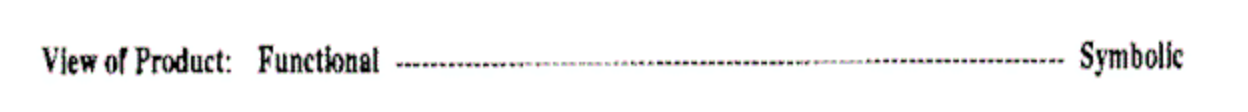
\includegraphics[width=1.19\linewidth]{function-symbolic.png}
  \caption{Fournier's spectrum of Meaning}
  \label{fig:function-symbolic}
\end{figure}
\vspace*{1.2em}

We want to classify objects into different categories of meaning.
Susan Fournier (1991) \cite{fournier1991} established a spectrum of meaning ranging from functional to symbolic.
From interviews with designers (Giacomin, 2017) \cite{giacomin2017} three categories of meaning emerged, function, ritual and myth.
Instead of symbolism, myth was identified as a category of meaning, and a third category emerged in between.
Unlike Fournier’s model however, the three terms were not intended to exist on a spectrum.
One hypothesis is that these classes can be mapped to product attributes and reverse-engineered in the design process of a product to elicit desired emotional responses in users.
This report covers the phase of our research process where we explored different means of gathering related words to function, ritual and myth with the purpose of finding descriptors that appear in everyday language and non-expert vocabulary.

Because we will use these related words in remote interviews with different groups of people, we need to increase our chances of effectively communicating our intended meaning of these words, and decrease the possibility of other people’s misconception.
Function can be associated with mathematics, computer science, biology and more.
Ritual and myth are more abstract and difficult to define in the context of human-artefact interaction.
We will need strong synonyms or even alternatives if we use these terms in interviews.

This report begins with an exploration of thesauri before moving to the search for a corpus of everyday language.
It continues with an exploration of ways to get related words from these corpora about our three focus words.
Finally, the results are compared against ready-to-use online tools for NLP.

%===================================

\chapter{Dictionary Definitions}

The initial process of gathering definitions, synonyms, antonyms and other related words was manually combing through various established dictionaries and online references and to collect the terms in a table.
The table in Figure \ref{fig:table1} represented below is an abbreviated version showing the breadth and range of results and not the full scope.
The full version is available at \href{https://meaning.pub.}{meaning.pub}.

\vspace*{1.2em}
\begin{figure}[!htbp]
  \hspace*{-3.666em}
  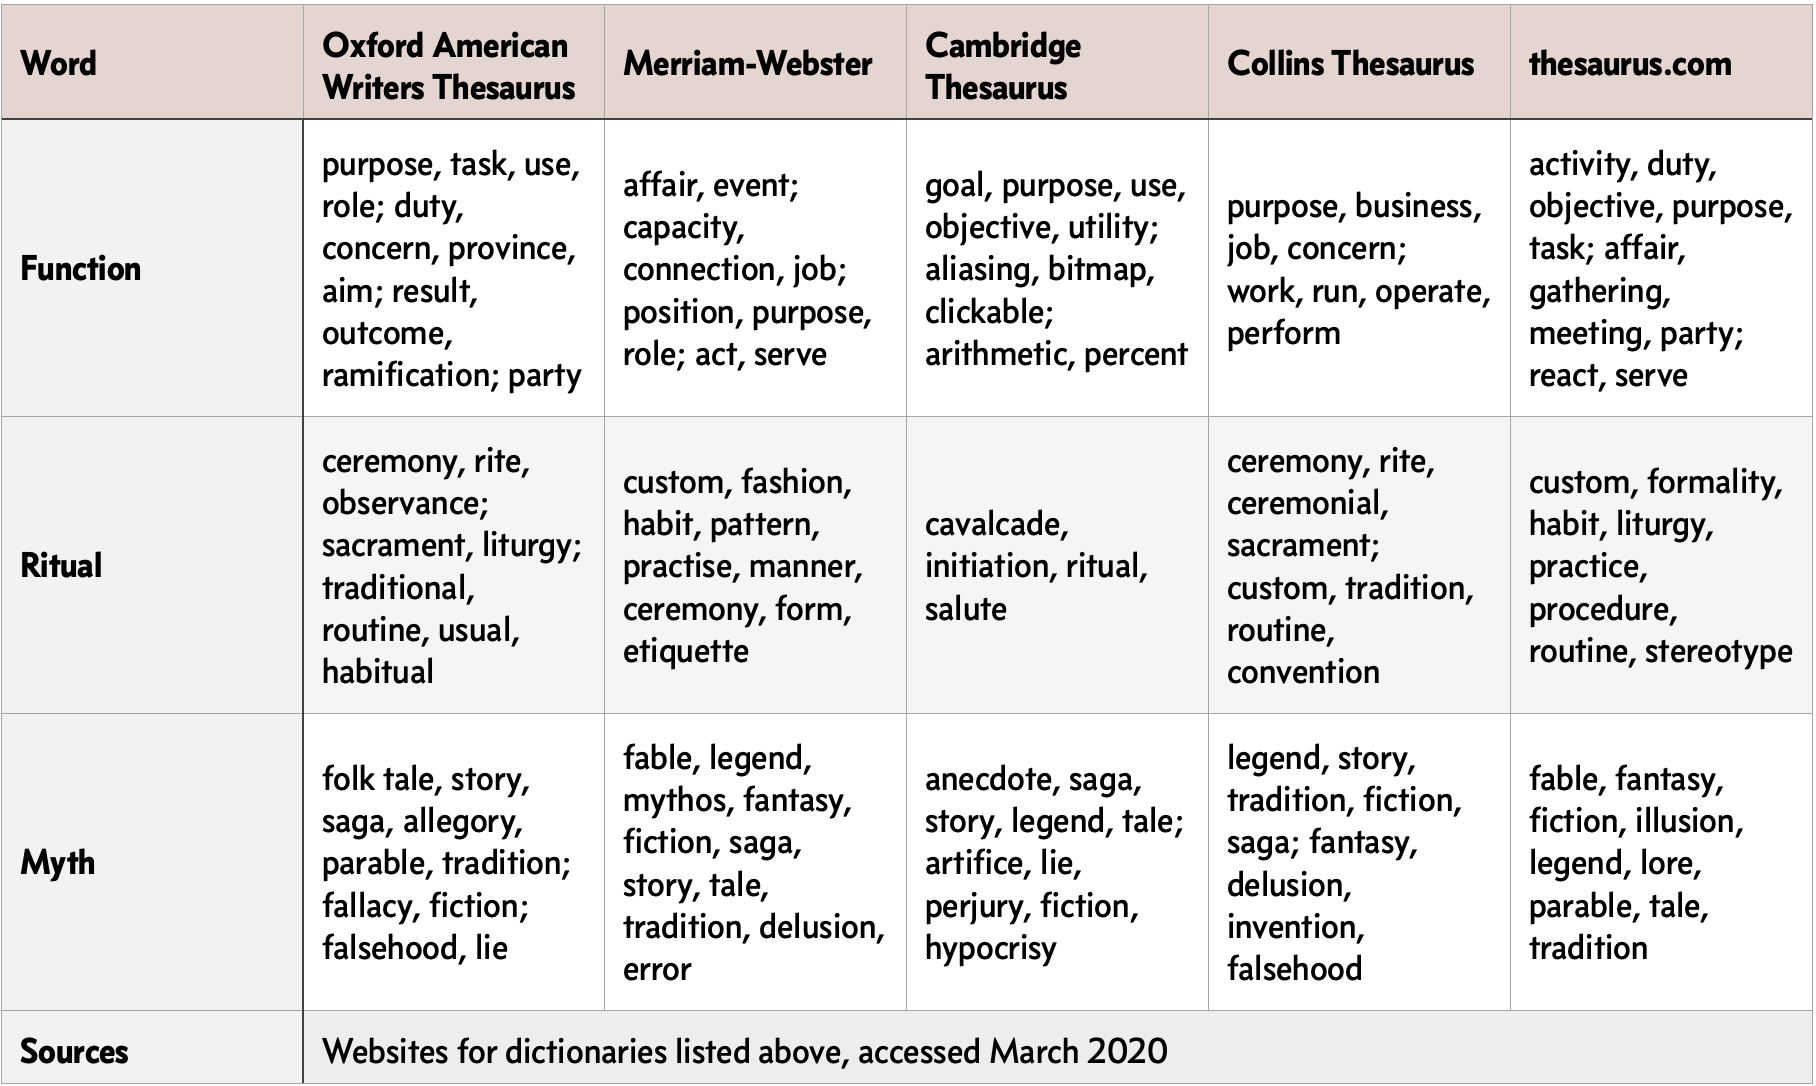
\includegraphics[width=1.19\linewidth]{table1.png}
  \caption{Related Words list --- a summarised range of results from selected dictionaries. the full table is available on our research website \href{https://meaning.pub.}{meaning.pub}.}
  \label{fig:table1}
\end{figure}
\vspace*{1.2em}

In Table 1 we can identify some differences between dictionaries, but largely these volumes have similar patterns.
What can be concluded is that the vocabulary in these dictionaries is formal.
Most dictionaries include informal variants of a word, but usually only one at the end of a long list of more formal terms.

Compiling the complete table of definitions and related words was a tedious and poorly scaleable process.
It is simple not efficient to manually read one dictionary at a time and write down the definitions and synonyms of a word.
The problem is also that the dictionary is becoming a rare book in the home and people will rather go to Google for their questions.
The dictionary is the wrong kind of reference if we want to establish today’s language.
If we want to build a real understanding of natural language used by non-experts, we need to extract the descriptors people use from a different, more casual corpus.

%===================================

\chapter{Corpus Search}

In Figure \ref{fig:table2} we compare different corpora used by computer scientists and linguists for extraction of natural language.
These corpora feature samples from written and spoken English (and other languages), and in some cases are already trained or annotated with vectors to be understood by machine learning programs.

\vspace*{1.2em}
\begin{figure}[!htbp]
  \hspace*{-3.666em}
  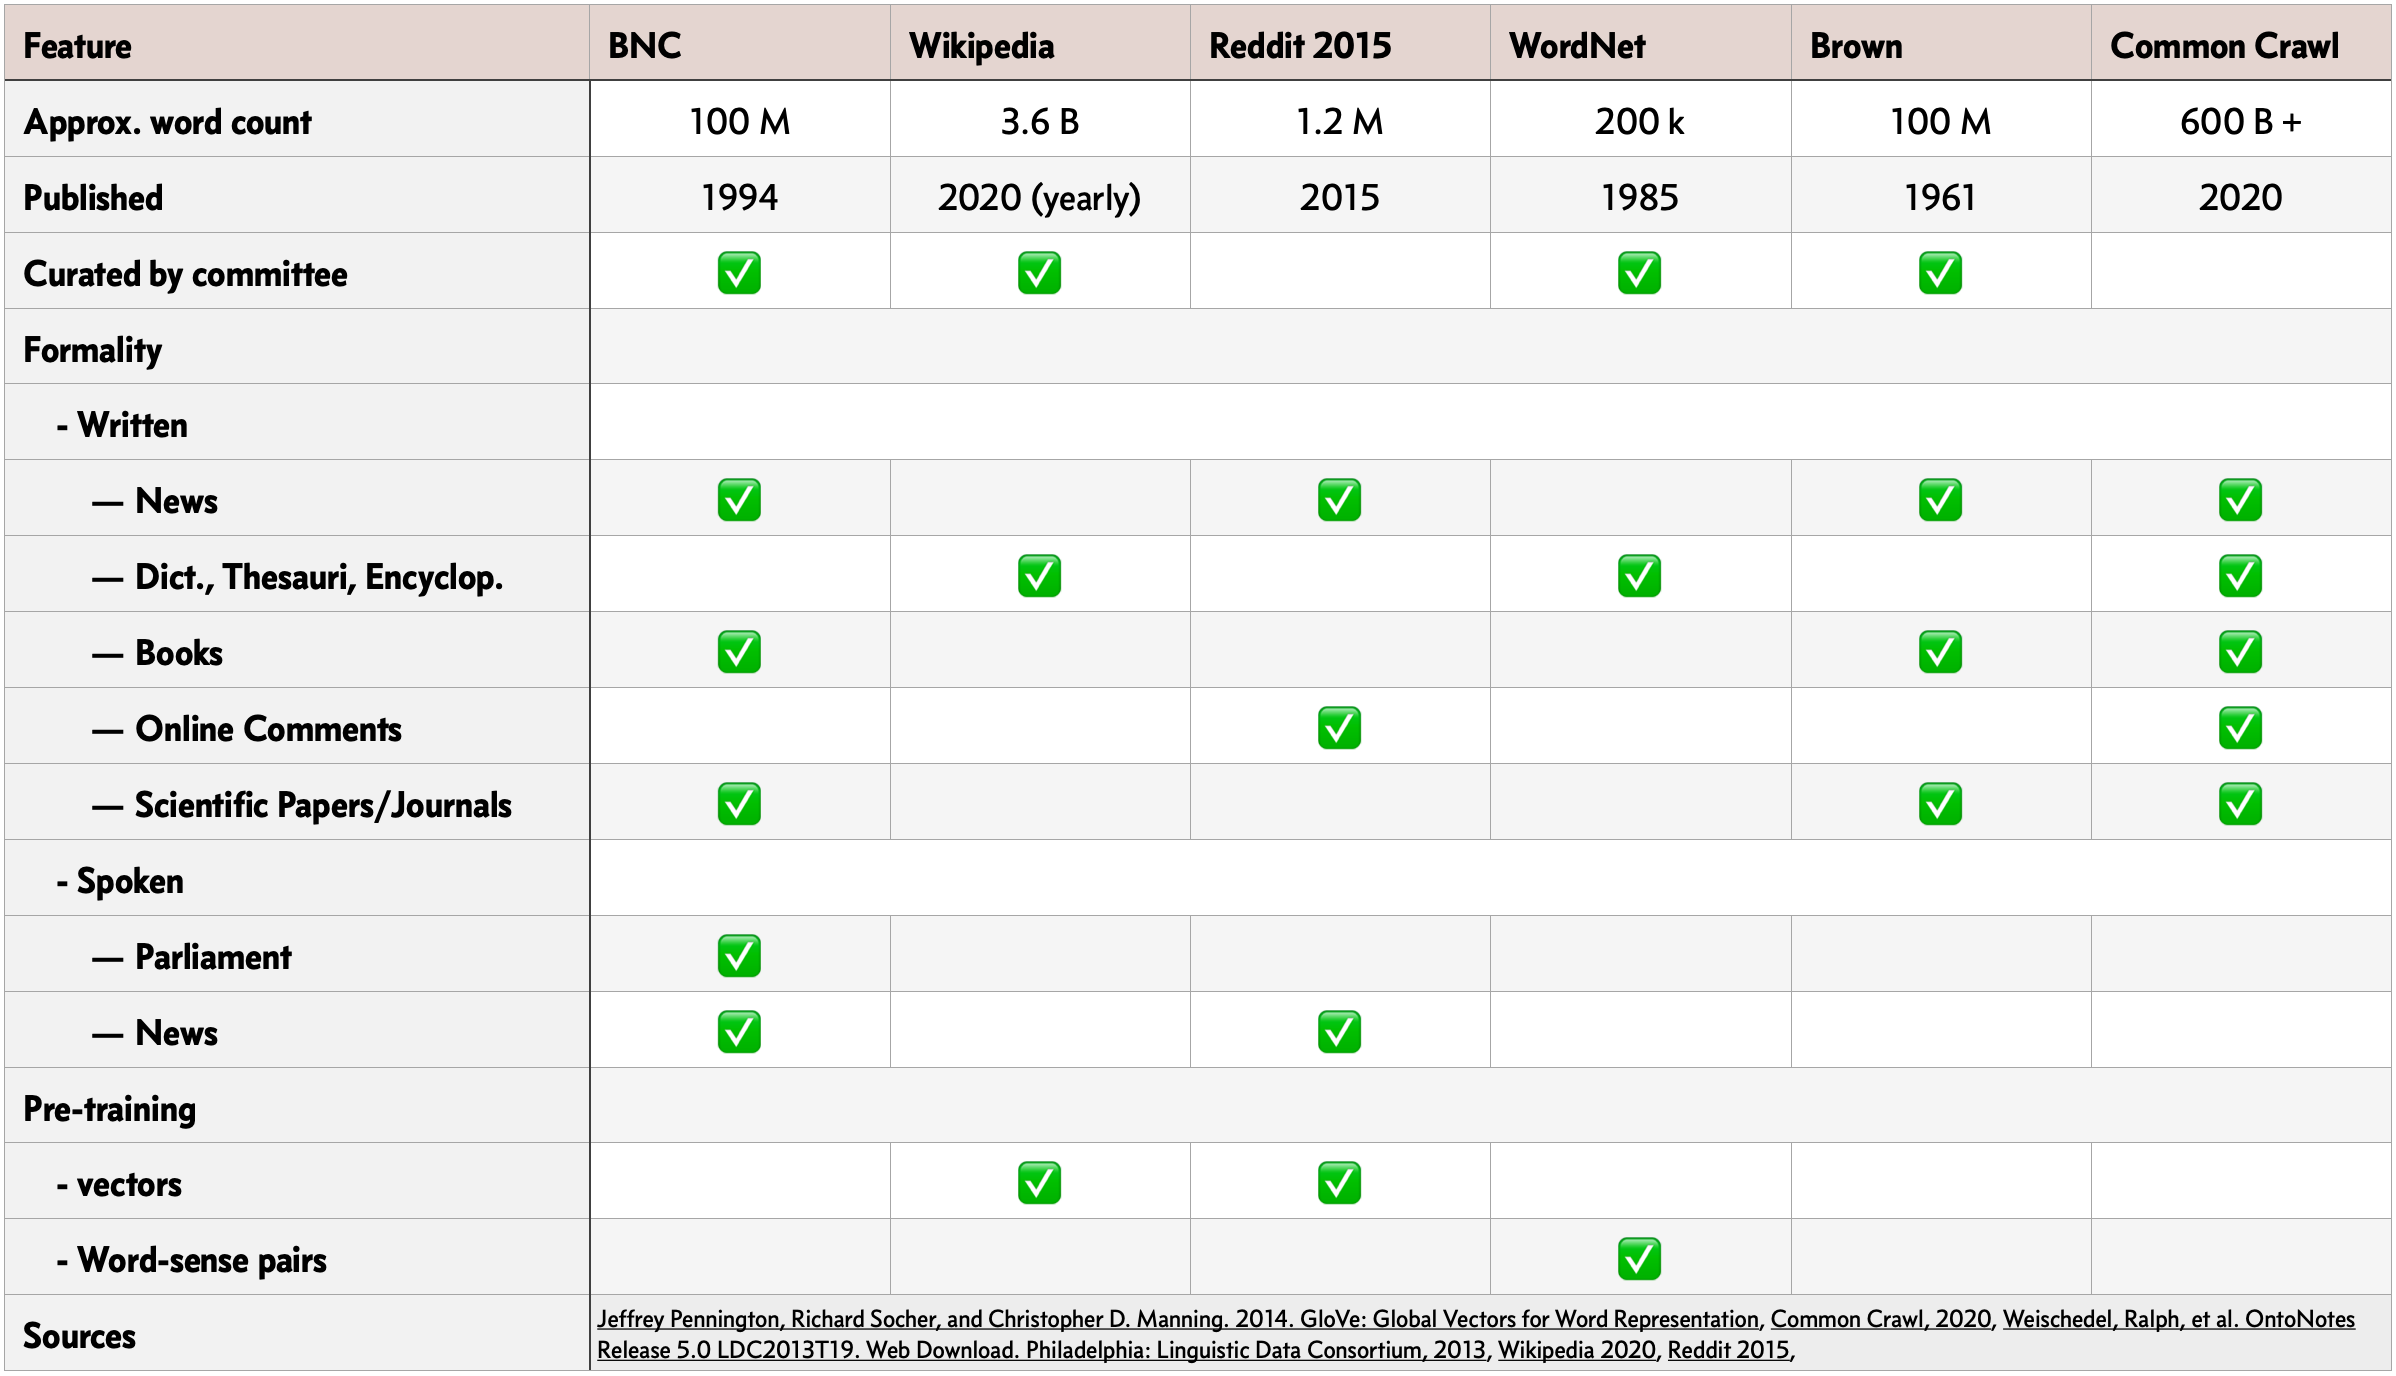
\includegraphics[width=1.19\linewidth]{table2.png}
  \caption{Comparison of selected corpora}
  \label{fig:table2}
\end{figure}
\vspace*{1.2em}

Some of these corpora are on the formal side of the spectrum, similar to our dictionaries.
The contents of these corpora are curated by a committee and contain peer-reviewed journal articles.
On the other side of the spectrum, we have informal corpora such as Reddit or Common Crawl.
These merely scrape an entire website (or in the case of Common Crawl the entire web) and collect all content.
This includes misspellings, made-up words, neologisms, derogatory speech, slang, acronyms and more.
While this may seem undesirable at first, the lack of a committee to filter content can also provide us with the most precise picture of naturally-used language by people.
Our desired corpus should feature a mixture of formal and informal samples, with a focus on the more casual, as we already have the dictionary data for a formal, recognised dataset to compare results against.
Using the right corpus, we can build a semantic network of related terms and explore the relationship of different words with our three focus words.
To build this network we will look at natural language processing, which combines machine learning and linguistics to give a computer the ability to process, analyse and understand language.
The different types of machine learning algorithms are defined by their context of use, their approach to problem solving and the data they process.
The defining factor for the quality of the output is the quality of the input.
We need to select
a good corpus. This corpus should be versatile enough to include the context we want, but also know about other contexts so that our model can learn what to ignore.
It will at first be used to train our model with a given algorithm and later we can plug our trained model into a new corpus to see how well it detects our desired words and if it can find new previously undiscovered terms.

%===================================

\chapter{Natural Language Processing (NLP)}

NLP focuses on expressing language in a way that is intelligible to machines.
It combines the power of linguistics and computer science to study the rules and structures of language, and create intelligent systems capable of understanding, analysing, and extracting meaning from text and speech (MonkeyLearn, 2019)\cite{monkeylearn2019}.

The field dates back to Alan Turing and his eponymous benchmarking test (1950)\cite{turing1950}.
Early applications were in translation work (IBM, 1954, ALPAC, 1966)\cite{hutchins2004}\cite{committee1966language}, rudimentary psycho-analytical chat bots (Weizenbaum, 1966)\cite{weizenbaum1966} and conceptual ontologies or knowledge graphs (Powers, 1984)\cite{powers1984}.

With the advent of machine learning in the 1980s, there was a revolution in the training of NLP models --- away from hand-curated rules, to an approach based more on probability and “learning by doing”. Machine learning algorithms learn automatically through experience (Mitchell, 1997) \cite{mitchell1997} and build a model based on a dataset.
Using this model, the algorithm can recognise statistical patterns and make predictions.

With part-of-speech tagging (POS tagging is the process of identifying words as nouns, verbs, adverbs, etc.) and the introduction of large text corpora (Brown, 1961, WordNet 1985) \cite{brown1979} \cite{wordnet1995} it became possible to build functioning machine translation models.
The next evolution came with word embeddings.
The next sections give a brief overview of the current standards in NLP.

%===================================

\section{Word Embeddings}

Corpus-based semantic representations (word embeddings) use statistical patterns in the text to map words in a vector space (Altszyler et al., 2017) \cite{altszyler2017}.
In the semantic word-space, terms with a similar meaning tend to form a cluster.
This relies on the concept that words with similar meaning appear in similar contexts (Harris, 1954) \cite{harris1954}.

Depending on the algorithm used to calculate the embeddings, different features (Figure \ref{fig:table3}) are used.
This is where the field becomes too opaque for us to offer a precise explanation, so we focused on what we can explain.

[Figure \ref{fig:table3} on next page]

\vspace*{1.2em}
\begin{figure}[!htbp]
  \hspace*{-3.666em}
  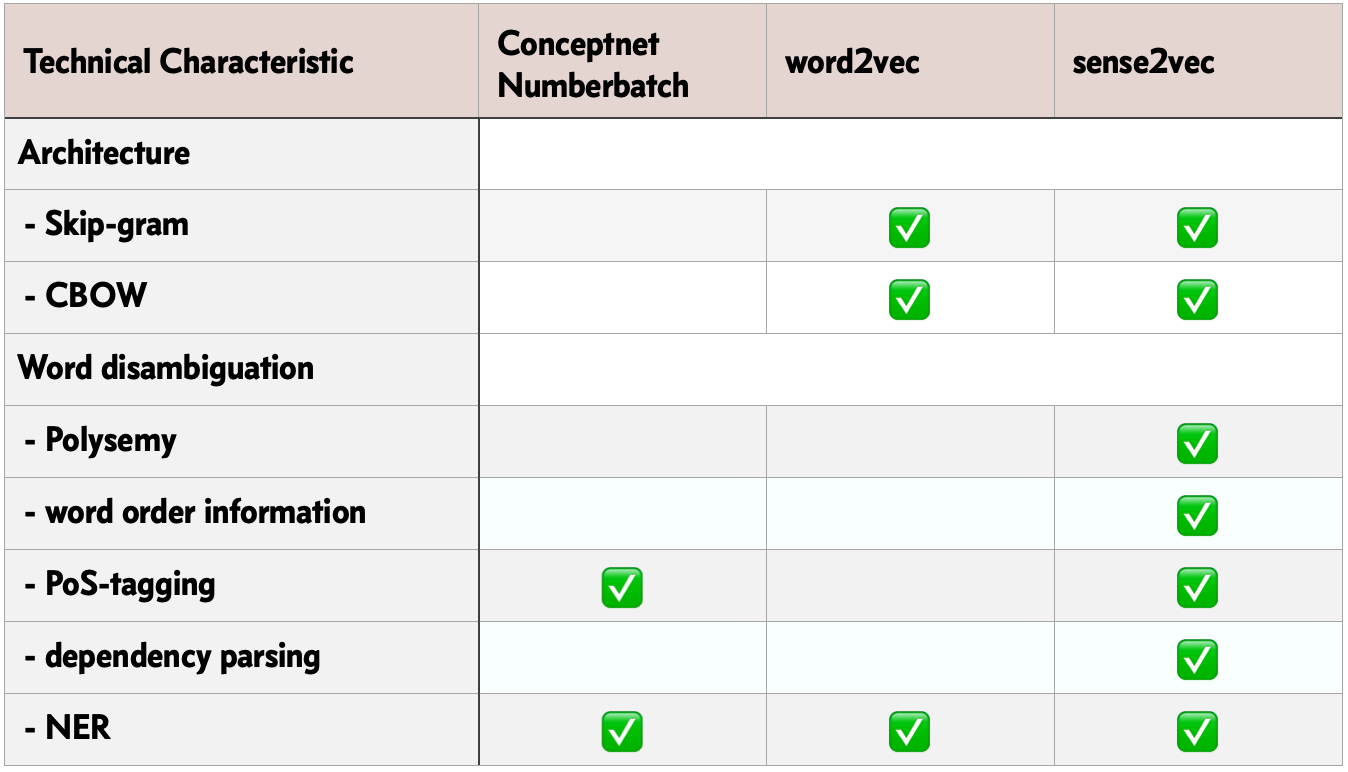
\includegraphics[width=1.19\linewidth]{table3.png}
  \caption{comparison of selected algorithms}
  \label{fig:table3}
\end{figure}
\vspace*{1.2em}

Named-entity resolution, or NER, parses a collection of words that belong together as one, for example New York City, or Pablo Picasso.
This entity is assigned a vector, rather than its individual parts.

Polysemy is the disambiguation of words with multiple meanings.
This has to do with POS, but is more nuanced since it looks at the context in which a word is used.
Two words can have the same spelling, same POS but different meanings.
Function is a good example.
Are we talking about a social gathering, the role at a company or the operation of a device? Here, each meaning, or sense, is assigned a unique vector.

Dependency parsing is the representation of words’ relation on each other, recognising the syntax of a sentence and learning about subject, object and action.

The two main architectures for word embeddings are CBOW (Continuous Bag-of-Words) and Skip-Gram.
In the CBOW architecture the goal is to output a focus word from a number of surrounding context words.
In the Skip-Gram architecture, our input is the focus word and we want to maximise the probability of outputting the context words.

%===================================

\section{word2vec}

Word2vec (Mikolov et al., 2013) \cite{mikolov2013} is used to produce word embeddings.
It takes words from a corpus and produces a vector-space with hundreds of dimensions, each word having their unique vector.
Words that are related by context in the corpus are located closely in the word-vector-space.

To get better results, Mikolov et al. describe a subsampling method to counter the imbalance in a data set between frequent words (“to”, “and”) that are not telling us anything unique about our input, and rare words which are more valuable in guiding the model.

In the Skip-Gram model, each word is defined based on the characters that compose it (its spelling) and is assigned a vector, a direction of meaning, capturing their semantic and syntactic information (Maas \& Ng, 2010) \cite{maas2010}.
That means that function, ritual and myth are assigned an individual vector, but also functions, functional and functionality, because these words are all spelled differently.
In word2vec, polysemous words share a same vector.

%===================================

\section{sense2vec}

The work by Reisinger \& Mooney (2010) \cite{reisinger2010} takes a new approach on vector-space word-sense disambiguation by first clustering the contexts in which a word appears to then encode multiple meanings, or senses, for polysemous words.
The methods of Chen et al.\ (2015) \cite{chen2015} or Rothe and Schütze (2015) \cite{rothe2015} use Princeton’s WordNet to find the number of definitions a word has instead of looking at a preset number of clusters.
These additional steps improve the quality of the output, but at the cost of heavier computation (Trask, 2015) \cite{trask2015}.

Sense2vec uses POS-tagging (Horn, 2017) \cite{horn2017} as well as named-entity resolution (NER) to assign each meaning of a word their own lexical unit.

%===================================

\section{NLP Libraries}

A library (or tool) combines the features of one or more algorithms and lets us plug in corpora to do our training and data analysis on.

\vspace*{1.2em}
\begin{figure}[!htbp]
  \hspace*{-3.666em}
  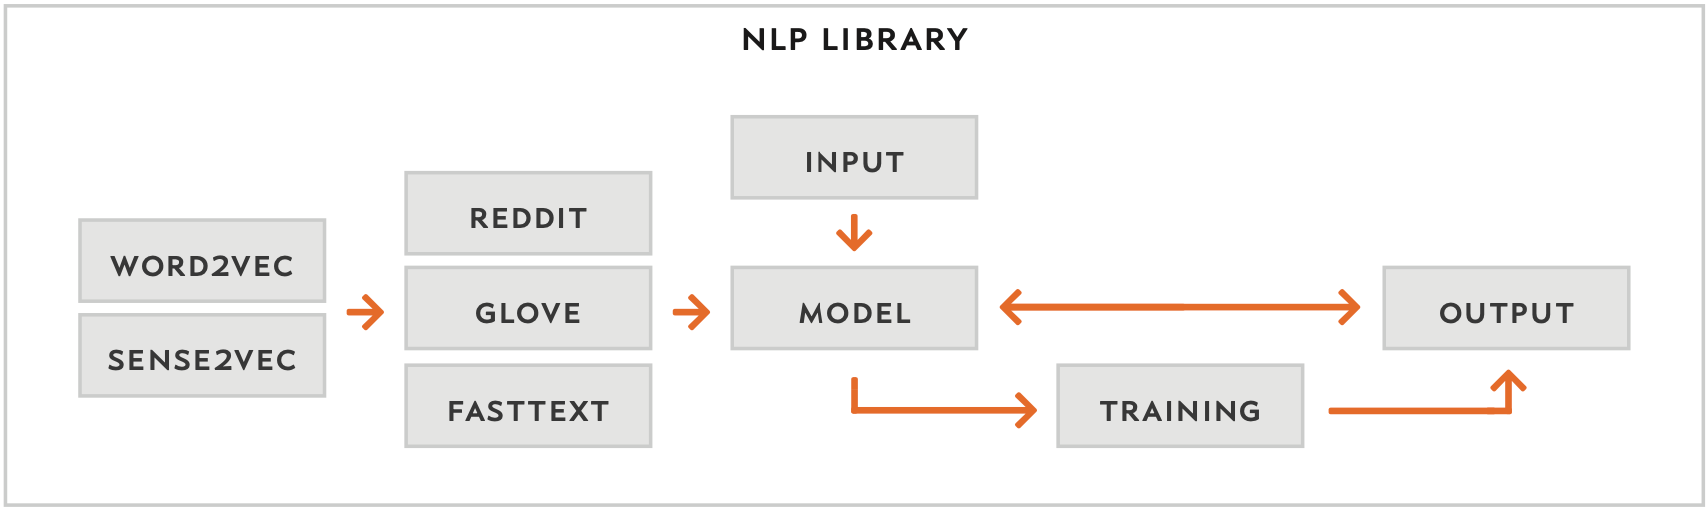
\includegraphics[width=1.19\linewidth]{fig1.png}
  \caption{Flowchart of library's function}
  \label{fig:figure1}
\end{figure}
\vspace*{1.2em}

Figure 1 outlines the function of a library.
It uses a word embedding algorithm to preprocess a corpus to be fed into a model.
This corpus can be vectorised or raw text.
An input word or document can be added to the model as a seed.
This can be enough to provide an output.
However, the result may not be in the desired word-vector space (context) and further training may be required.
The back-and-forth between model training and output evaluation may have to be repeated for a dozen instances before desired results are visible.

NLTK is one of the most-recommended libraries, however it is quite large and not obvious to the beginner.
For us, it is crucial that we use a production-ready library, as we cannot invest the time to learn multiple tools.
If one library provides good documentation in the form of tutorials and can be used on its own, it becomes a viable candidate for our selection.
We also established that we need sense2vec in our algorithms as it will theoretically provide more intelligent results.
The sense2vec architecture also offers polysemous word-sense disambiguation, which is crucial to differentiate between the different meanings of function.

Lemmatisation can reduce derivations of a same word (word, words, wording) to its stem, or lemma.
All possible derivations of a word’s lemma make up the lexeme of this word.
Stemming is similar, but also takes into account conjugation or pluralisation where the spelling or a word changes completely.

We want the library to have a simple way of training.
Since the words we are using can exist in many contexts, we will want to guide the model in the right direction.
This can be done by evaluating the output and repeating the process with trained data.
We are currently seeing this stage as a potential source of poor results.

Other basic features of libraries include tokenisation, where each word and symbol in a sentence is identified as its own token, and classification, where words or named entities can be categorised into a common group like sports or economics.

\vspace*{1.2em}
\begin{figure}[!htbp]
  \hspace*{-3.666em}
  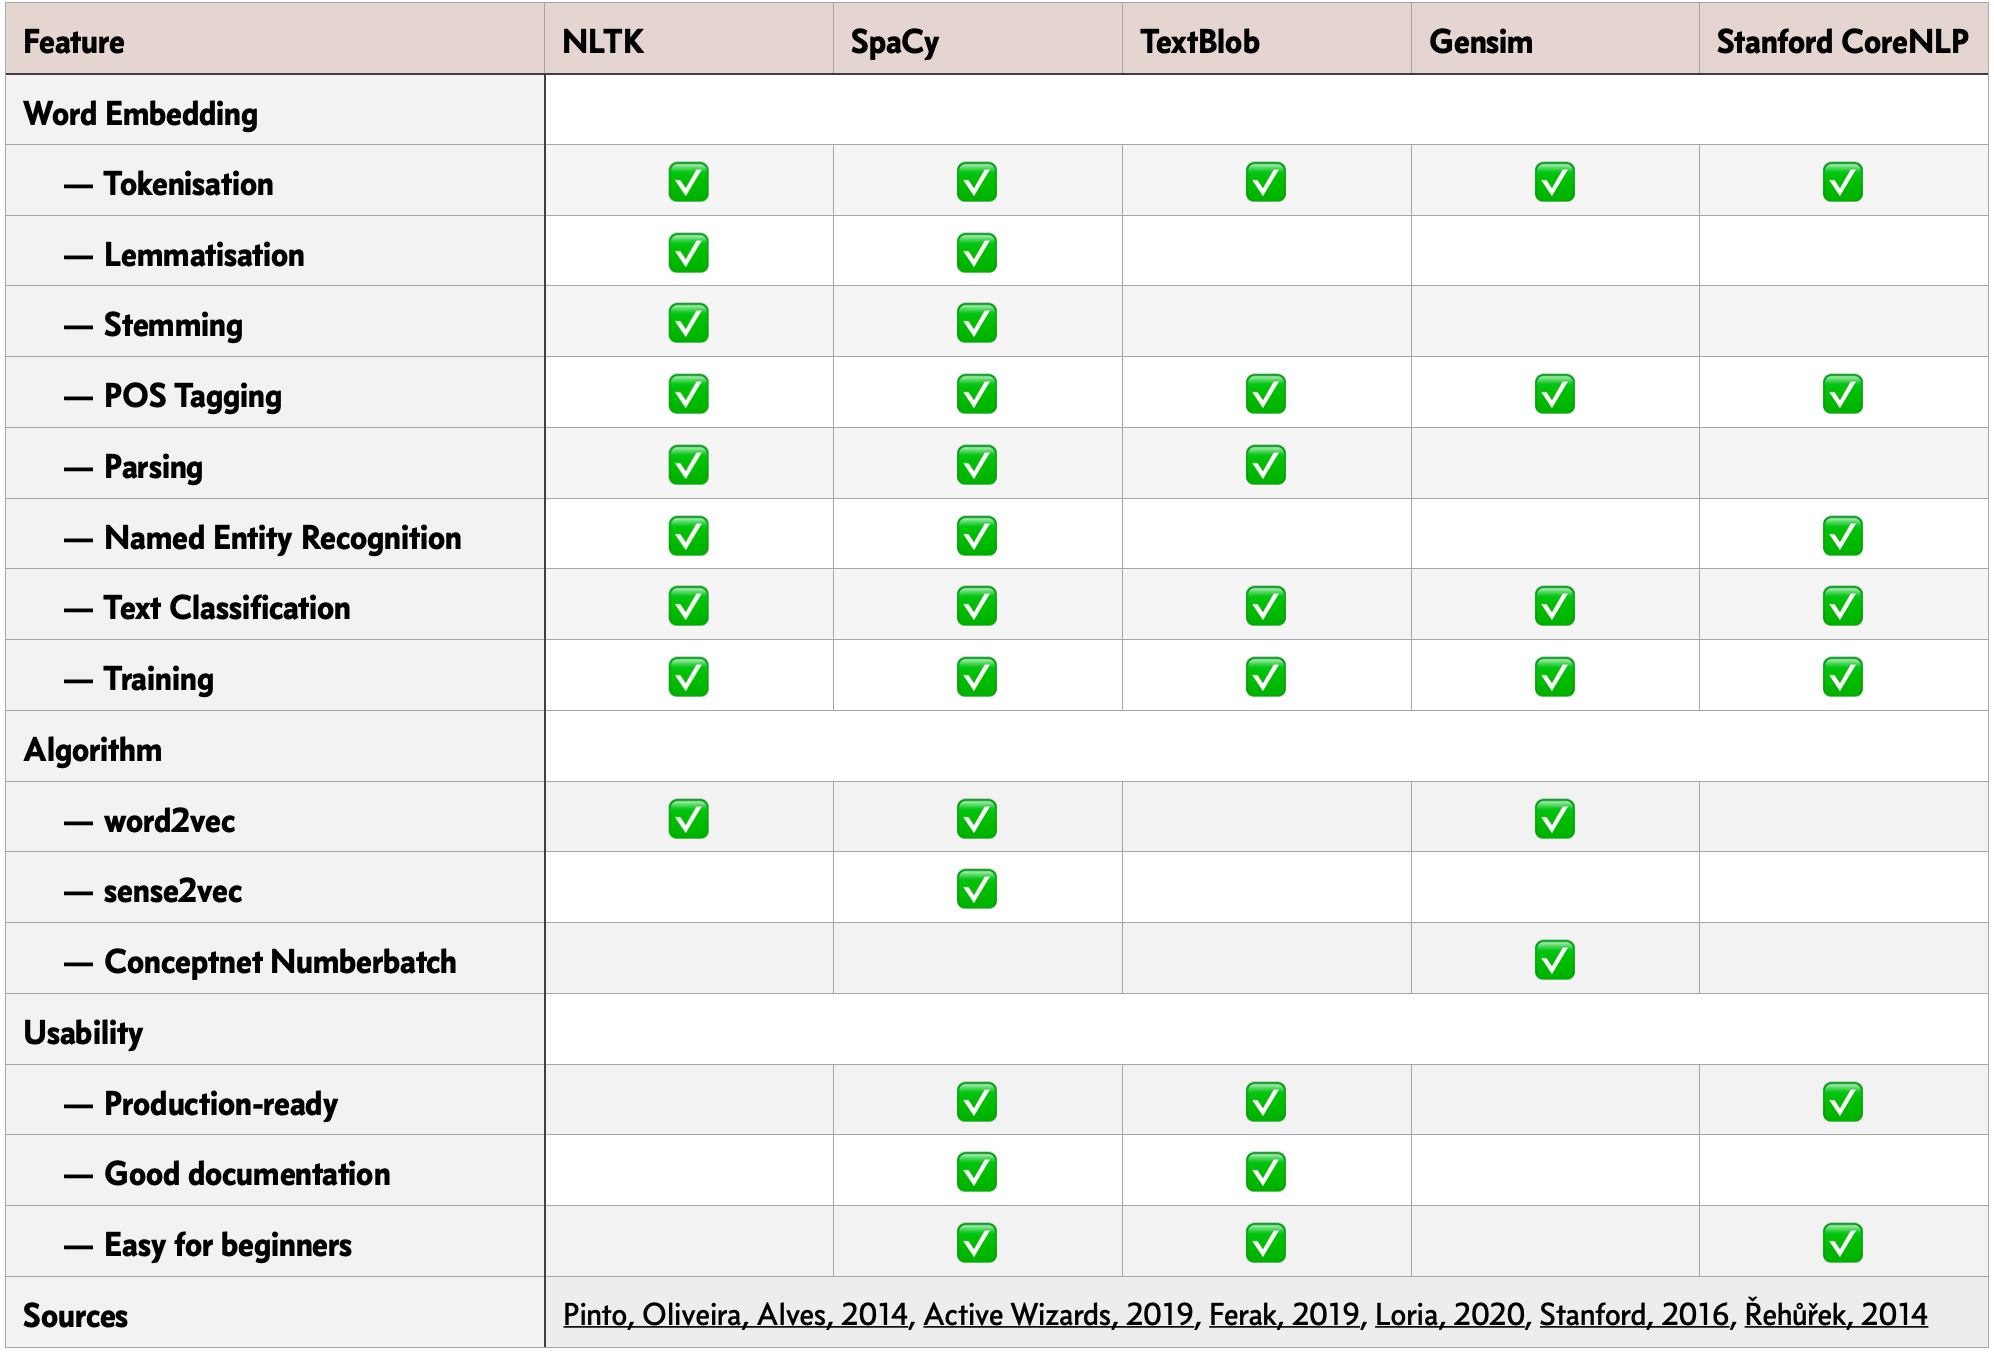
\includegraphics[width=1.19\linewidth]{table4.png}
  \caption{comparison of selected NLP libraries}
  \label{fig:table4}
\end{figure}
\vspace*{1.2em}

From Figure \ref{fig:table4} above, SpaCy can be identified as the most promising candidate.
It has most of the features and although it’s relatively new and not as established as NLTK, it has a comprehensive documentation along with tutorials that we can follow along to learn the tool.
From our research, it seems like a favourite among new NLP projects for its speed and ease of use.
The makers of SpaCy, Explosion, also have a text classification and training tool called Prodigy that can be used for text classification.
Text classification can help us identify senses of our focus words in a corpus.

In theory, once the model is sufficiently trained we can test results from different corpora and find related words based on context, from formal to informal.
So far, however, no results have been achieved that could beat those provided by online demos where we had no control over training the model to focus on our desired word-vector space.

We reached out to Explosion and they provided us with a free research license of Prodigy, a tool that would normally cost \$400.
We are currently still evaluating and learning Prodigy.
Once we produced results aligning with our goal, we will purchase the tool as to not appear biased towards the developers.

%===================================

\chapter{Results from NLP}
\section{Technique for online tools}

In parallel to comparing and selecting a good library for us to use we looked into ready-to-use tools to build semantic networks.
Since approached to NLP are problem-specific, there are no comprehensive programs with a user interface where we can select a corpus and receive output based on some input words. 
What we found were examples of application or proofs of concept by companies with tools that are up to the individual to design and program to their exact needs.
Examples such as those by Explosion (SpaCy), Turku University’s NLP Group, Google’s Tensorflow, a demo by Anthony Liu, or Radim Řehůřek (Gensim) have a setting to select vector dimensions or switch from CBOW to Skip-Gram, but mostly a simple input into a textfield will yield results.
Other examples such as ConceptNet or Facebook’s FastText required a small amount of programming in Python or depended on Gensim to function and parse the vectors.

\subsection{ConceptNet}

ConceptNet is a freely-available semantic network to find related words in its ontological multi-lingual database from Open Mind Common Sense, Wikipedia, WordNet, etc and was developed by Speer et al.\ (2017).
When searching for a word, the results are displayed in classes --- synonyms, related terms, types of, derived terms, ways of, things used for, context of, word forms, etymological relatives, antonyms and more.
The tool understands different levels of dependency, can detect if a word has an effect on another word and what the use of the word is.
Depending on the input word, the quality of these dependencies and related words varies widely.
Figure 2 is a screenshot from ConceptNet website, comparing results for x is capable of illustrating the differences when looking up regular words versus rare words.
With decreased frequency of use the models have a hard time understanding the relationships the word has on others.
The results from ConceptNet’s website are output in all languages it can find related words for.
This overcrowds the results.
ConceptNet have a clearly-written API on GitHub with examples of related word queries filtered to English and including or excluding certain parameters.
The given parameters for a word can be viewed in the API.
The complete semantic network for myth can be viewed at api.conceptnet.io/c/en/myth.
This pattern matches for all word queries.

\vspace*{0.2em}
\begin{figure}[!htbp]
  \hspace*{11em}
  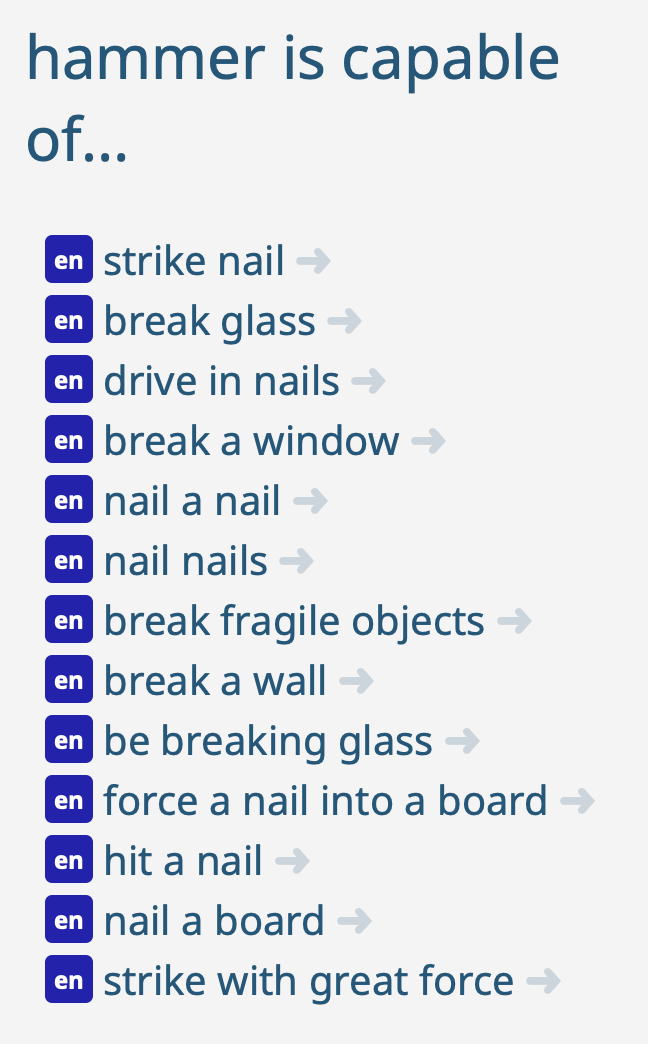
\includegraphics[width=0.4\linewidth]{fig2.png}
  \caption{ConceptNet example results for \emph{Hammer}}
  \label{fig:figure2}
\end{figure}
\vspace*{0.2em}

We wrote a script that gets the related words of our input term, removes the derived terms and forms of the word, and outputs the results in a table.
The API calls in our script are humanly-readable and go as followed:
First, we get the related words using \lstinline{http://api.conceptnet.io/related/c/en/alpha}, where alpha is our input word.
Then we call derived terms \lstinline{http://api.conceptnet.io/query?node=/c/en/alpha\&rel=/r/DerivedFrom} and forms of \lstinline{http://api.conceptnet.io/query?node=/c/en/alpha&rel=/r/FormOf} and subtract both from the related words list.
The difference is output into a table which we copied into Table 5 in section 4.3 on page 17.
We also attached weighting to the related terms, the meaning of the weighting however is not qualifiable, nor is a low weighting an indicator for uninteresting words.
We wrote the script to have flexibility over the number of output words and compared the results with 10, 20 and 50 output words per term.
The results were poor with 10 results and we did not gain further insight looking at 50 results.

\subsection{Turku University’s NLP Group}

Turku University in Finland have an NLP department which maintains an online demo of word2vec trained on 4.5 billion Finnish words from the Finnish Internet Parsebank, a project which they describe with three goals:
First to create a tool with automatic syntactic analyses, second a complete classification database and third an online user interface to interact with, which is their demo in Figure 3.

\vspace*{1.2em}
\begin{figure}[!htbp]
  \hspace*{-3.666em}
  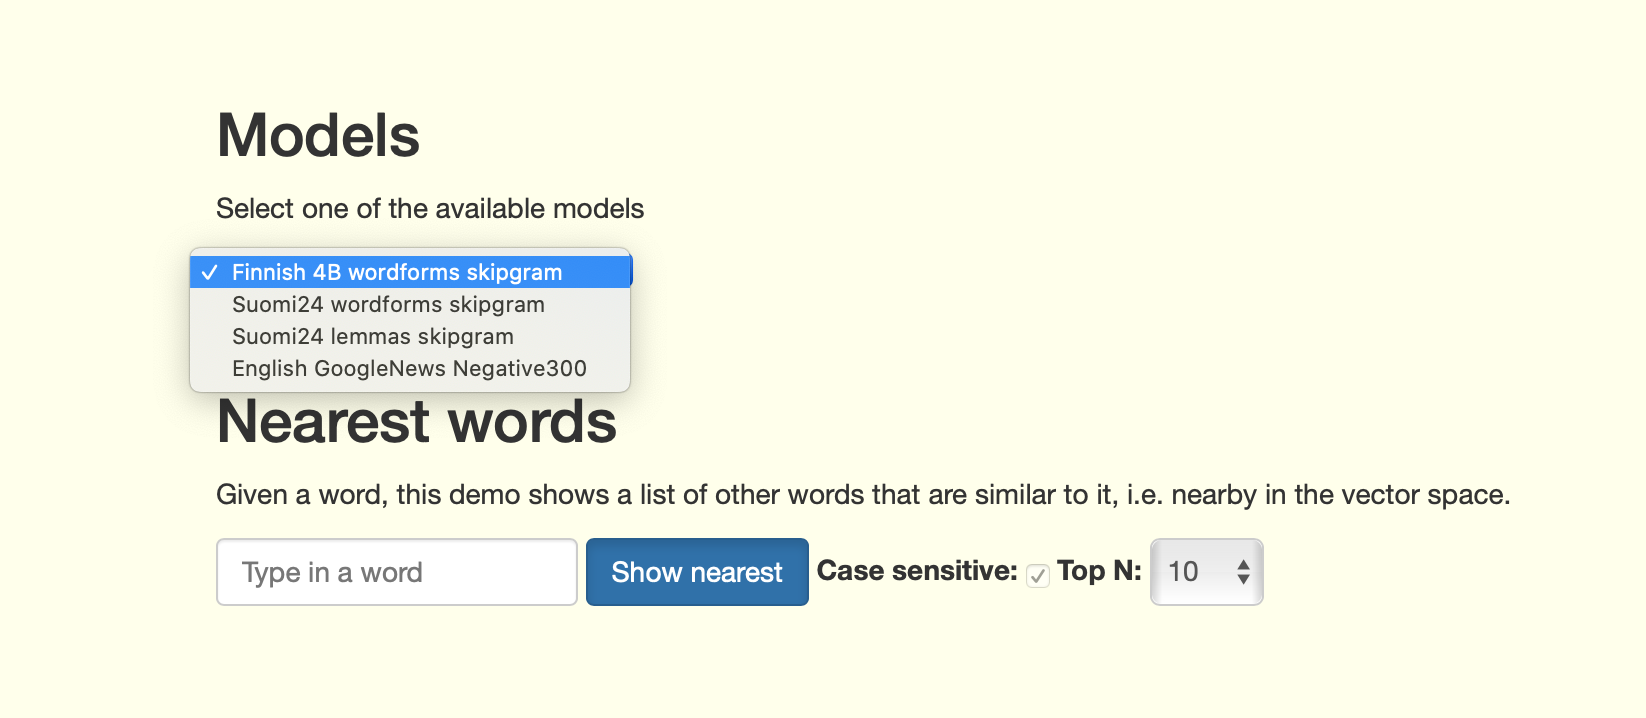
\includegraphics[width=1.19\linewidth]{fig3.png}
  \caption{Turku University’s NLP Demo at \url{http://bionlp-www.utu.fi/wv_demo/}}
  \label{fig:figure3}
\end{figure}
\vspace*{1.2em}

Their demo allows for the selection of different models and next to searching
for nearby words also offers the possibility to view the numeric similarity of two words and to compute a word analogy akin to word2vec's example king - man + woman $\approx$ queen (Mikolov et al., 2013) \cite{mikolov2013}.

We did not use the comparison or analogy features and instead focused on getting 10 related words for a single input word and repeated the process for each of our three focus words.
The results were copied into Figure \ref{fig:table5}).

\subsection{Anthony Liu’s demo}

We found another word2vec demo this time using common English words as a corpus.
It was created by Anthony Liu, an MIT computer scientist with a specific focus on theoretical neuroscience and AI.

\vspace*{1.2em}
\begin{figure}[!htbp]
  \hspace*{-3.666em}
  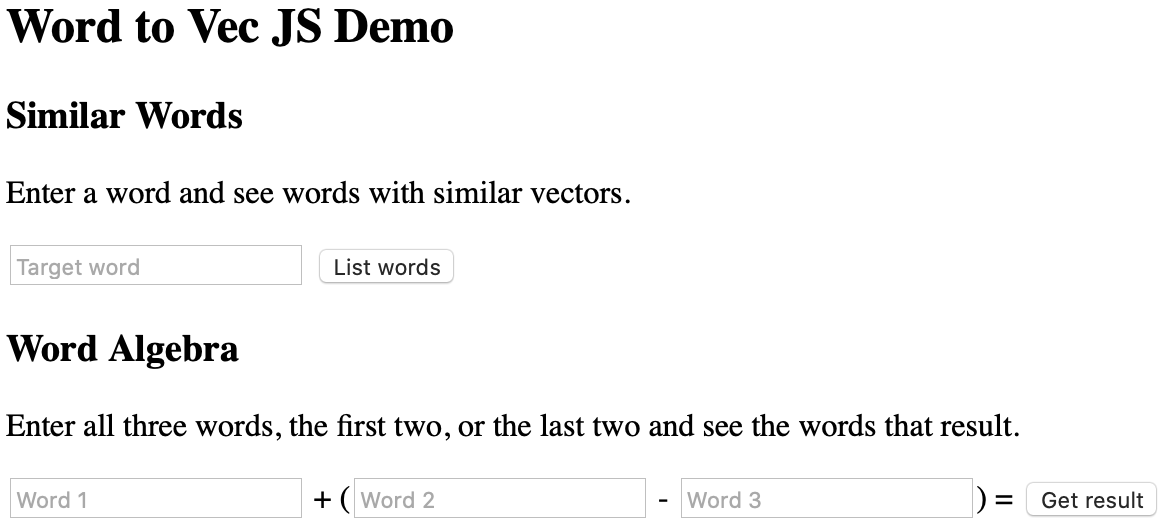
\includegraphics[width=1.19\linewidth]{fig4.png}
  \caption{Word to Vec JS Demo}
  \label{fig:figure4}
\end{figure}
\vspace*{1.2em}

This demo (Figure \ref{fig:figure4}) also has the option for word algebra which we forwent in favour of finding 10 related words.

\subsection{Gensim + FastText, Gensim + GloVe}

FastText by Facebook is a library for text classification.
It includes models with one million vectors trained on Wikipedia and two million on Common Crawl.

To use FastText, we had to include it in a Gensim wrapper as it doesn’t have a ready- to-use online demo.
GloVe is an algorithm by Stanford’s NLP department that also uses vectors trained on Wikipedia and Common Crawl, with 400.000 and 1.900.000 words respectively in its vocabulary.

Gemsim can be installed and ran in a Python script using import gensim.
We then loaded the the pre-trained FastText vectors from Wikipedia and later GloVe into Gensim with the command gensim.models.KeyedVectors. load\_word2vec\_format(‘vectors.vec’).
Then we output the 10 most similar results for our focus words using most\_similar(‘word’, topn=10).

\subsection{SpaCy + Reddit}

SpaCy’s developers, Explosion, have an online demo (Figure \ref{fig:figure5}) of sense2vec using the social discussion and news website Reddit.
In the demo it is possible to input a word and to specify its part-of-speech as well as which year to pick data from.
This lets people compare the change of meaning a word has over time.
The data available is form 2015 and 2019, so while there are no universal linguistic shifts in such a short period, it can be observed that occurances of the word trump now refer to the American President, when before it was linked to ranking.

\vspace*{1.2em}
\begin{figure}[!htbp]
  \hspace*{-3.666em}
  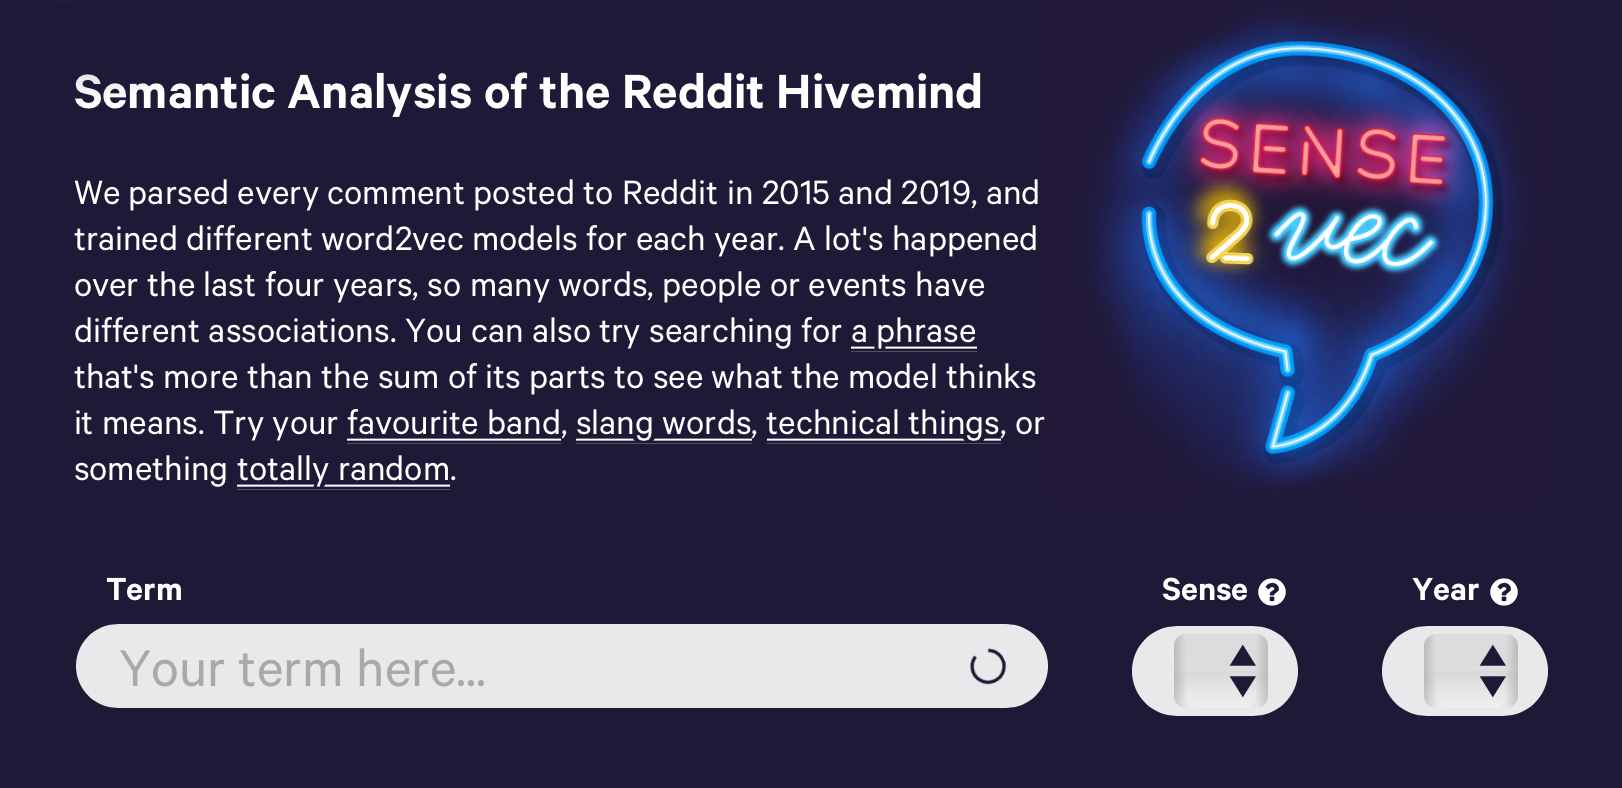
\includegraphics[width=1.19\linewidth]{fig5.png}
  \caption{sense2vec Demo}
  \label{fig:figure5}
\end{figure}
\vspace*{1.2em}

\subsection{Tensorflow Project}

The TensorFlow Embedding Projector by Google is an open-source tool for interactive 3D visualisation and interpretation of embeddings (Smilkov et al., 2016) \cite{smilkov2016}.
It is used to graphically represent high-dimensional embeddings and lets us visualise the relationship of words in our vector-space (Figure \ref{fig:figure7} on the next page).
The online demo we are working with uses a corpus of 25.000 movie reviews from IMBD, the internet movie database.
These movie reviews contain a wide variety of words without being too informal or technical.

We won’t get into details about their data visualisation attributes in this paper, more background information can be found in the paper published by Distill, a peer-reviewed scholarly online journal dedicated to machine learning research, “How to Use t-SNE Effectively” by Wattenberg et al. (2016) \cite{wattenberg2016}.

To read data, we searched for our focus words, increased the points to 1000 and switched to using t-SNE with the standard settings of 200 dimensions, a perplexity of 8, a learning rate of 10 and no supervision.
We let the calculations run for 8000 iterations.
From the table on the right in Figure \ref{fig:figure6}, we copied the 10 first results of nearest points into our results table (Table \ref{fig:table5}).

\vspace*{1.2em}
\begin{figure}[!htbp]
  \hspace*{-3.666em}
  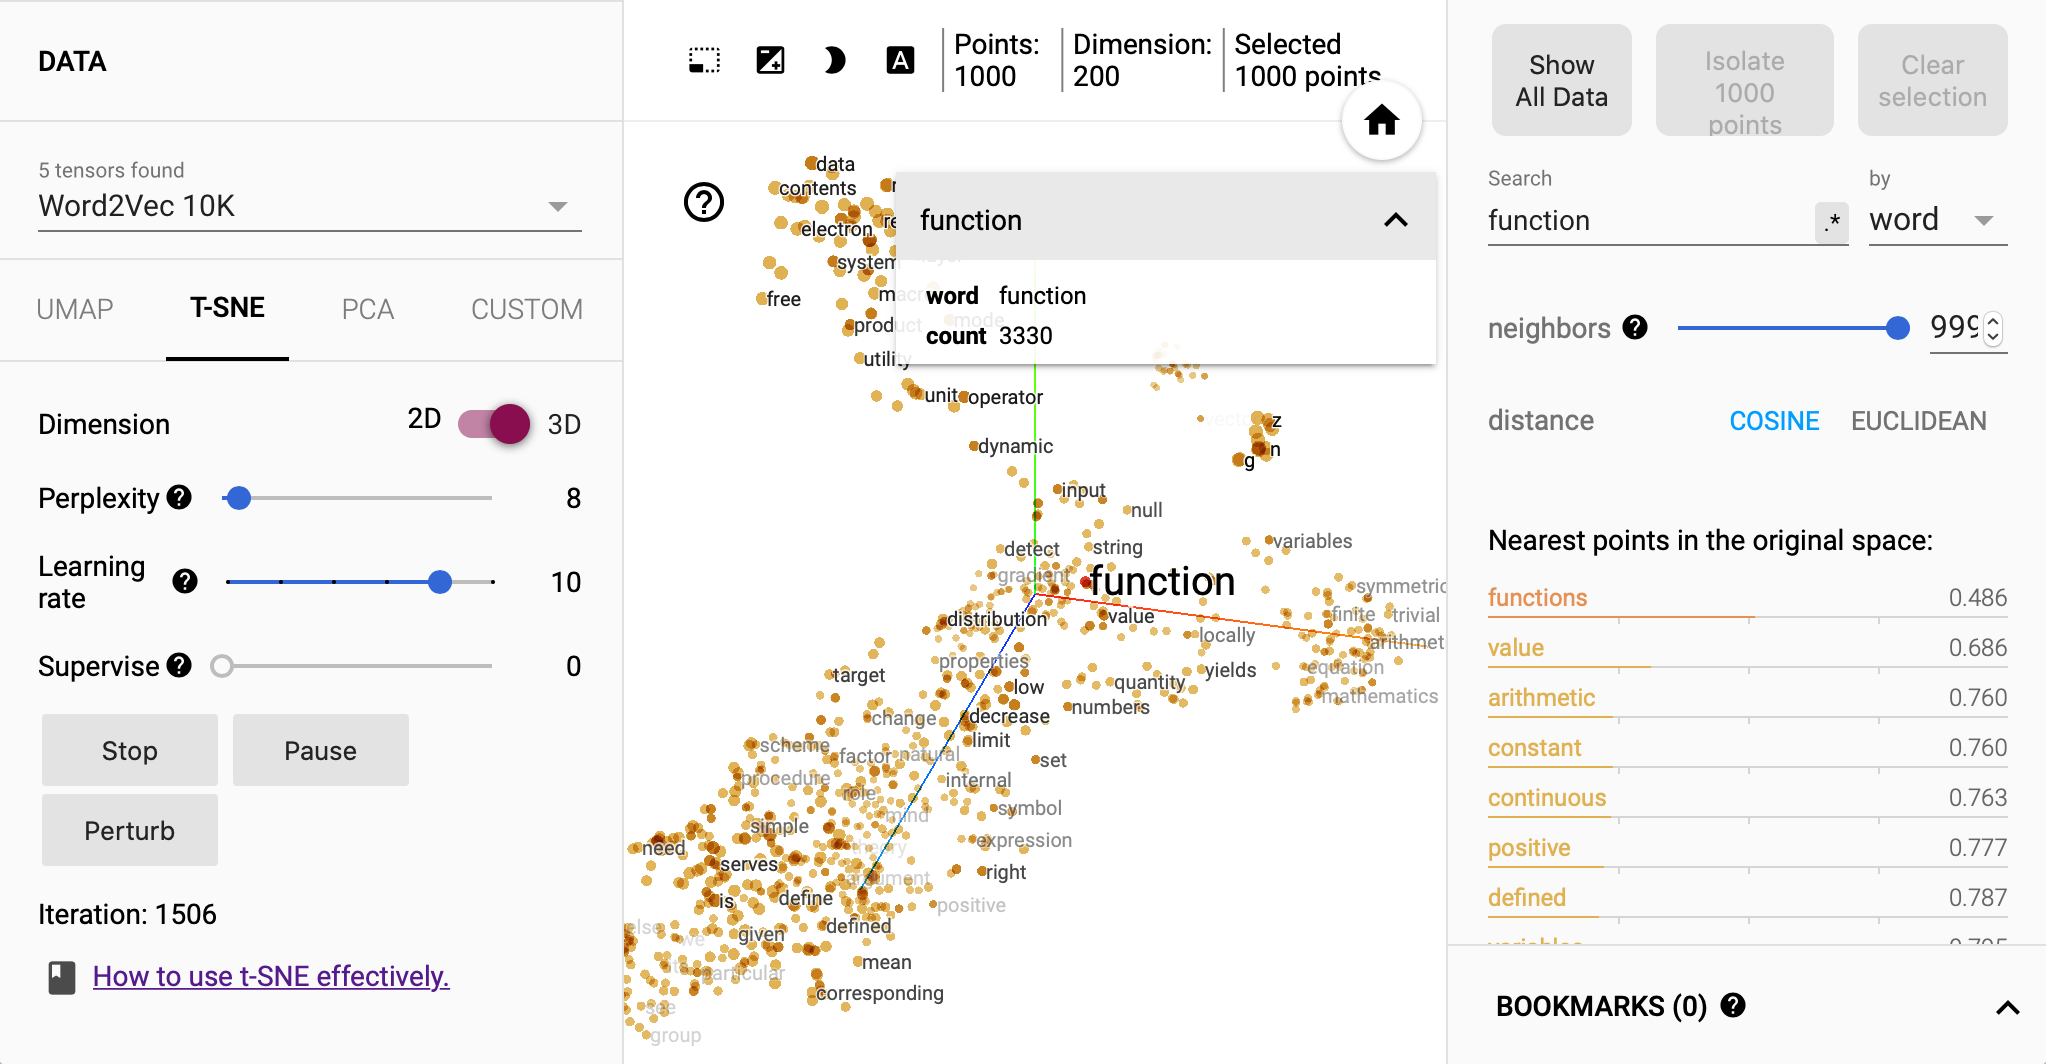
\includegraphics[width=1.19\linewidth]{fig6.png}
  \caption{Tensorflow Projector}
  \label{fig:figure6}
\end{figure}
\vspace*{1.2em}

From Figure \ref{fig:figure7}, \ref{fig:figure8} and \ref{fig:figure9} we can identify word clusters for our three focus words.
While some of these clusters are physically separated from the rest of the words for function and ritual, for myth there are no directly-visible outliers.

\vspace*{1.2em}
\begin{figure}[!htbp]
  \hspace*{-3.666em}
  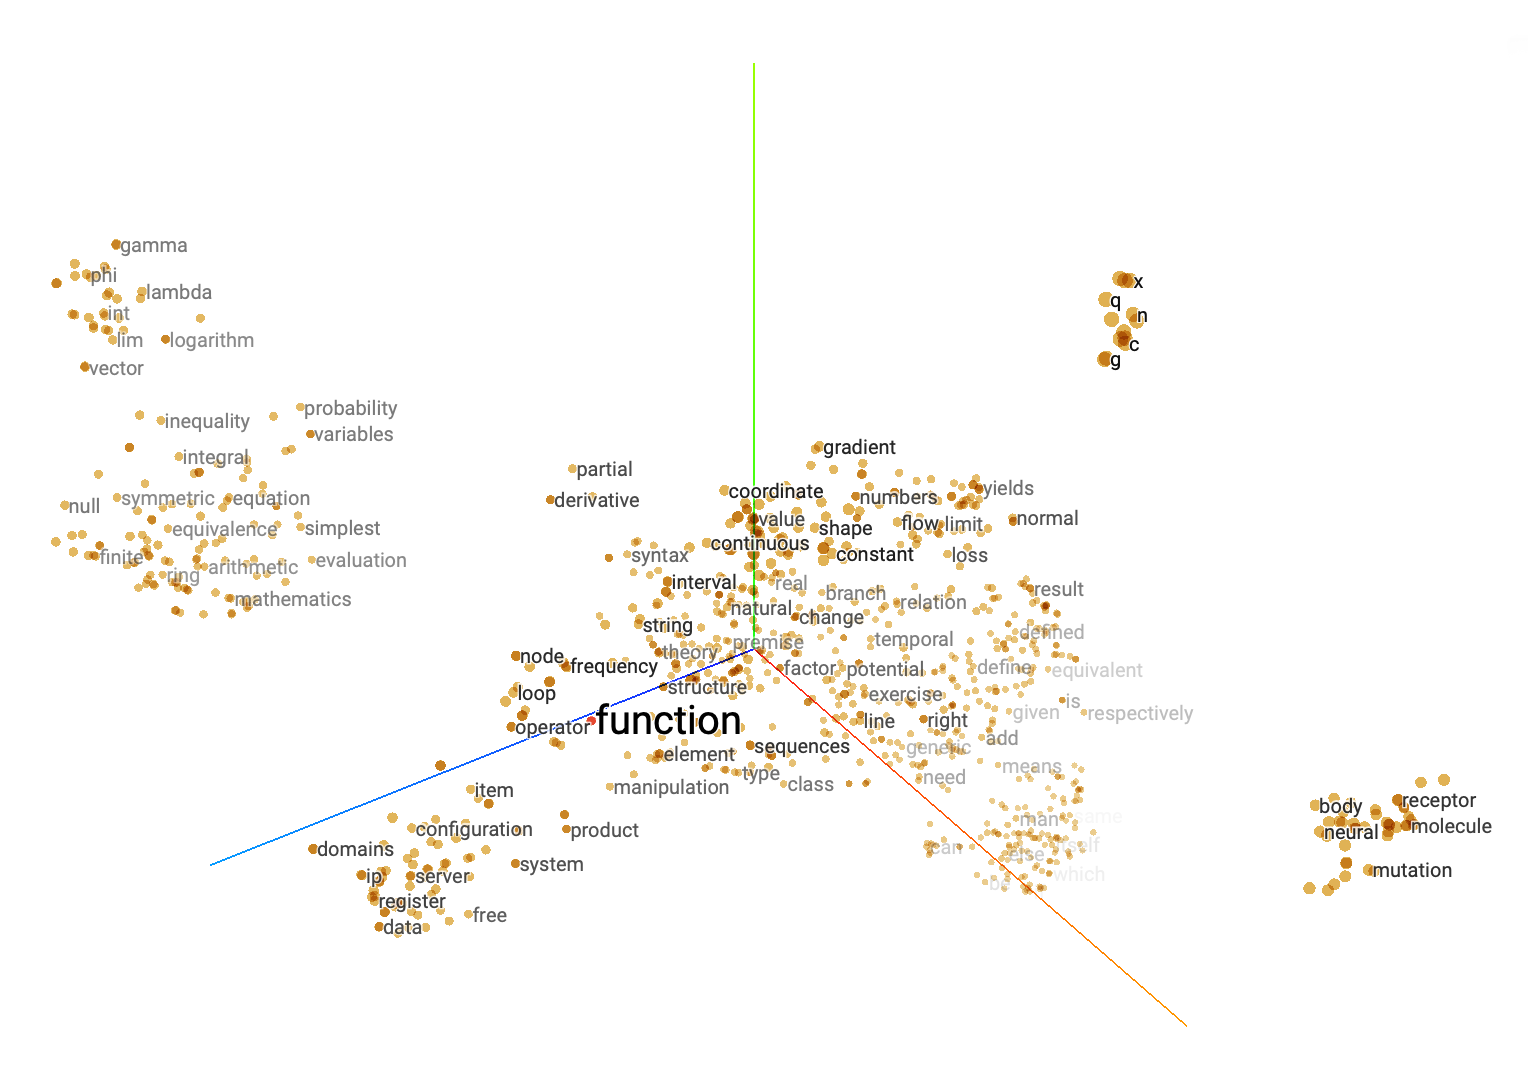
\includegraphics[width=1.19\linewidth]{fig7.png}
  \caption{Tensorflow Projector: Function}
  \label{fig:figure7}
\end{figure}
\vspace*{1.2em}

\vspace*{1.2em}
\begin{figure}[!htbp]
  \hspace*{-3.666em}
  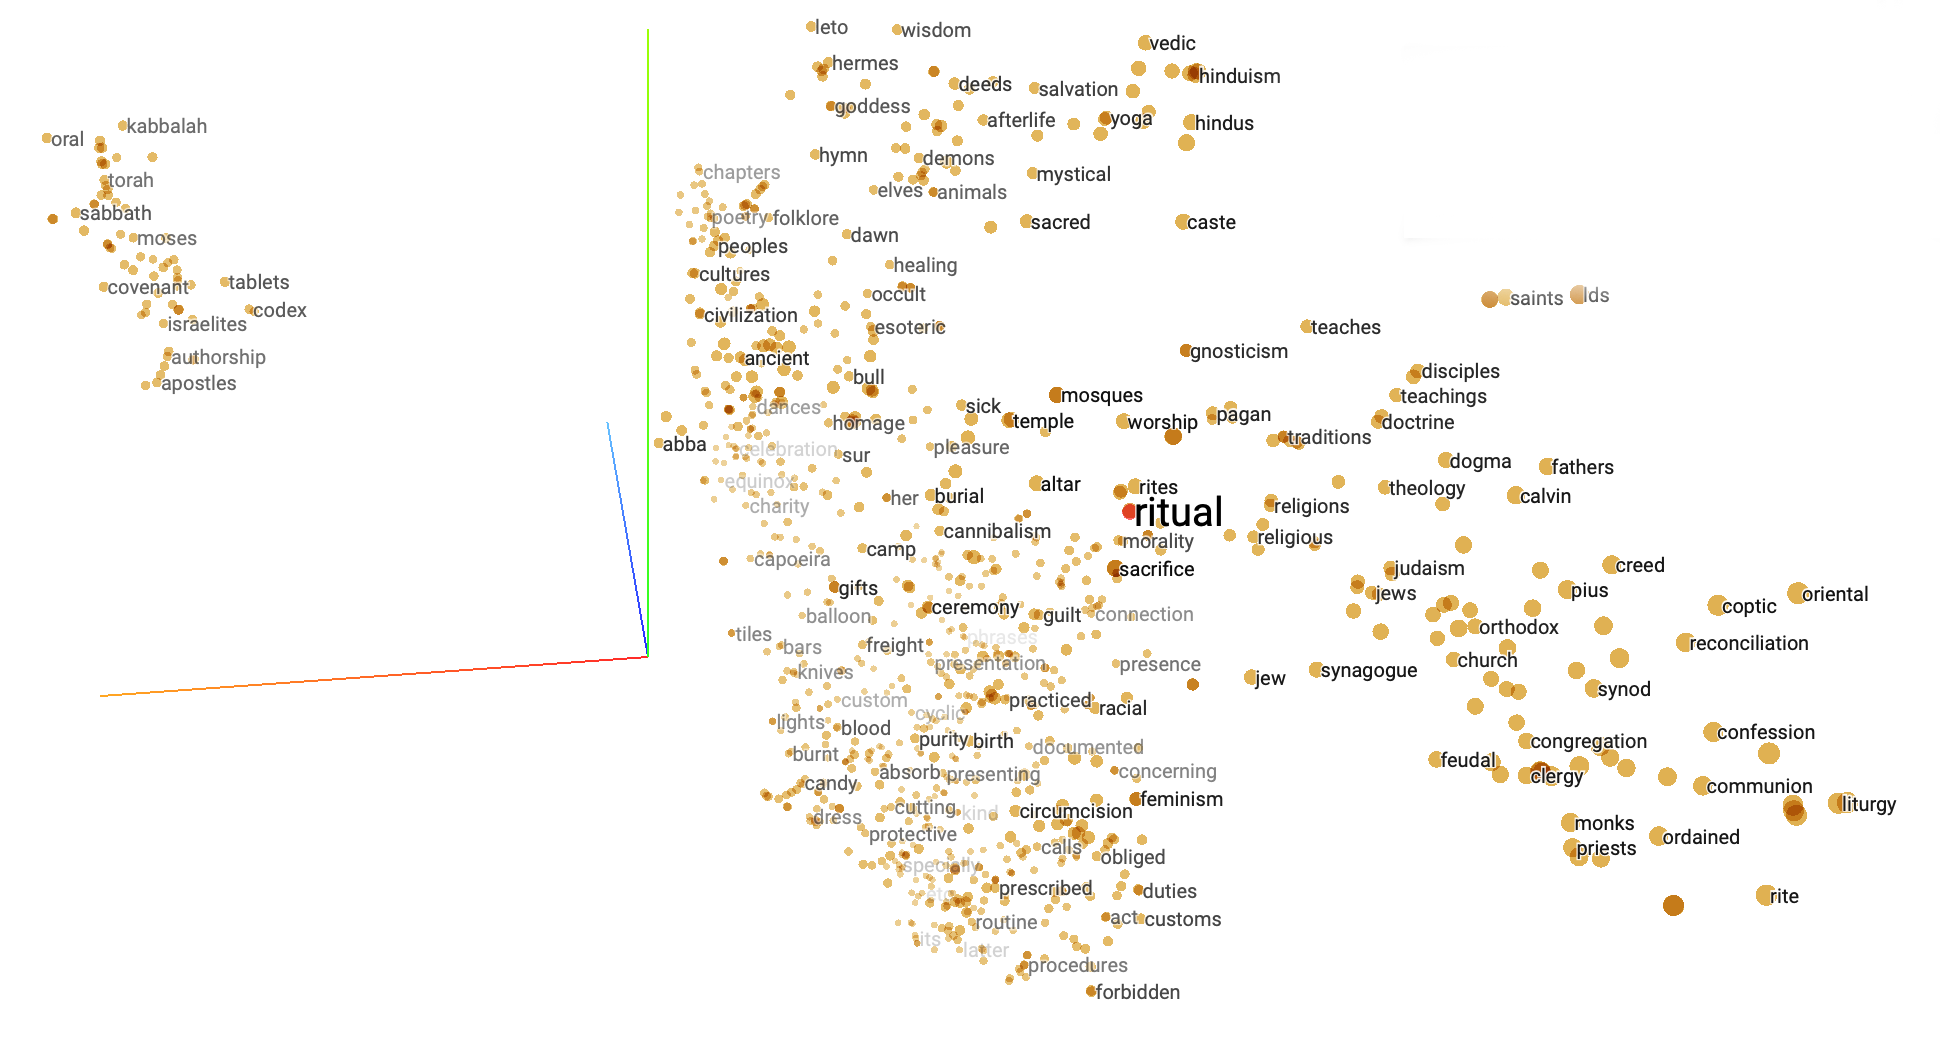
\includegraphics[width=1.19\linewidth]{fig8.png}
  \caption{Tensorflow Projector: Ritual}
  \label{fig:figure8}
\end{figure}
\vspace*{1.2em}

\vspace*{1.2em}
\begin{figure}[!htbp]
  \hspace*{-3.666em}
  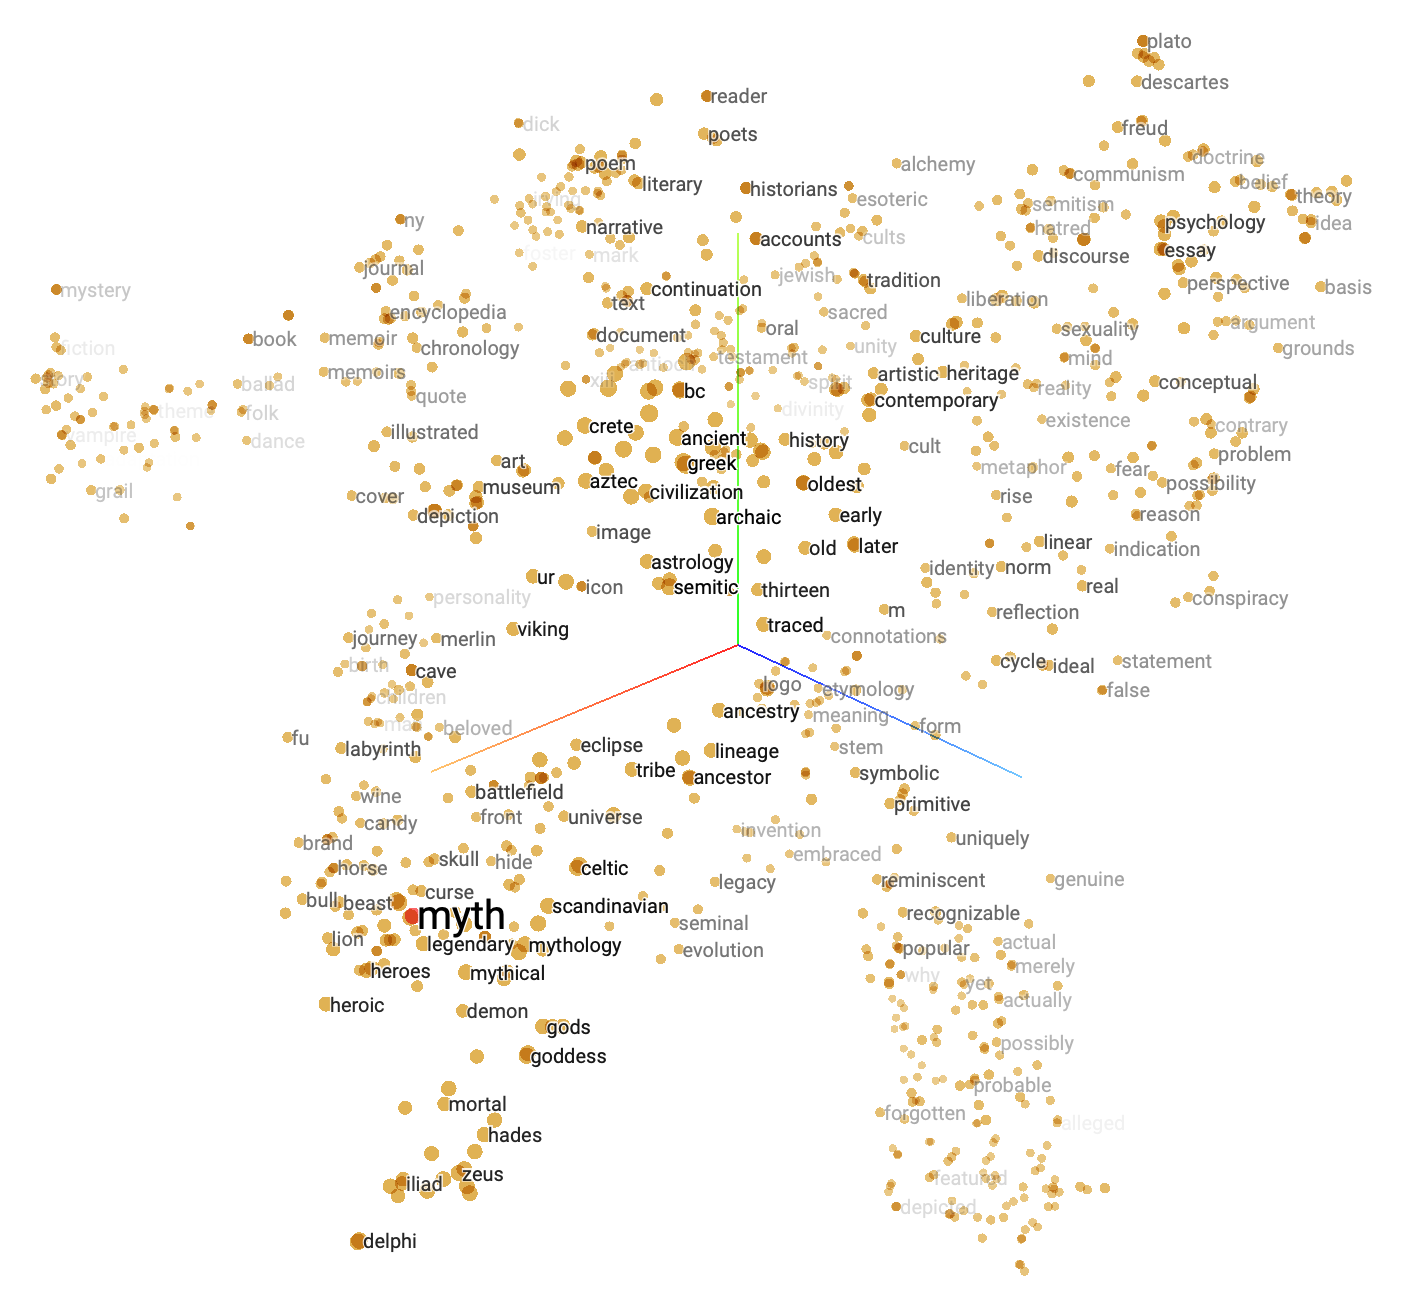
\includegraphics[width=1.19\linewidth]{fig9.png}
  \caption{Tensorflow Projector: Myth}
  \label{fig:figure9}
\end{figure}
\vspace*{1.2em}

\subsection{Polyglot}

Polyglot is another multi-lingual NLP library developed by Al-Rfou et al. (2013) \cite{alrfou2013} with an online demo available on Al-Rfou’s website.
It is not clear from our research if Polyglot is using word2vec for their word embeddings but since the results in Table \ref{fig:table5} vary from other word2vec models, we can assume Polyglot uses more intelligent word-sense disambiguation and handles polysemy as well as stemming and lemmatisation.

\vspace*{1.2em}
\begin{figure}[!htbp]
  \hspace*{-3.666em}
  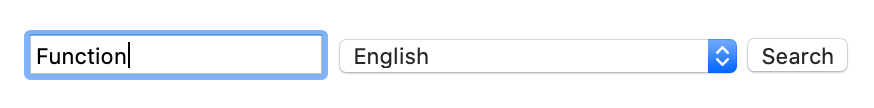
\includegraphics[width=1.19\linewidth]{fig10.png}
  \caption{Polyglot Demo}
  \label{fig:figure10}
\end{figure}
\vspace*{1.2em}

The demo does not have any visible settings (Figure \ref{fig:figure10}) except for language, where it loads vectors from the respective Wikipedia.

%===================================

\section{Technique for SpaCy}

SpaCy’s stand-alone training tool Prodigy was the focus of our NLP research as it checked all boxes in our library comparison and its features addressed everything we understood as being important.
The tool allows us to create a new word category and train a model to recognise words that belong in that category.
To use the word2vec and sense2vec models from SpaCy, we first had to install their tools into a virtual python environment, the details of which process can be read in our blog post about debugging the Prodigy installation.

Once we were set up, we could use the command prodigy terms.teach function\_pattern en\_core\_web\_lg --seeds function.txt to load the terms.teach recipe using the en\_core\_web\_lg model which contains OntoNotes5 and GloVe with 685.000 vectors and 300 dimensions.
The model was loaded with three seed terms (function, task, use) in our function.txt text file.
Prodigy launches a local web-server (Figure \ref{fig:figure11}) where we can graphically see the words to categorise and can accept, reject or ignore words.
We can also undo our classification and revisit a word.

For our results table (Table \ref{fig:table5}) we wrote down the first 10 words that we received from Prodigy without accepting or rejecting them.
This process was repeated for function, ritual and myth using a fresh pattern file for each, where training data is saved to and can be loaded from in a second round of text classification.

\vspace*{1.2em}
\begin{figure}[!htbp]
  \hspace*{-3.666em}
  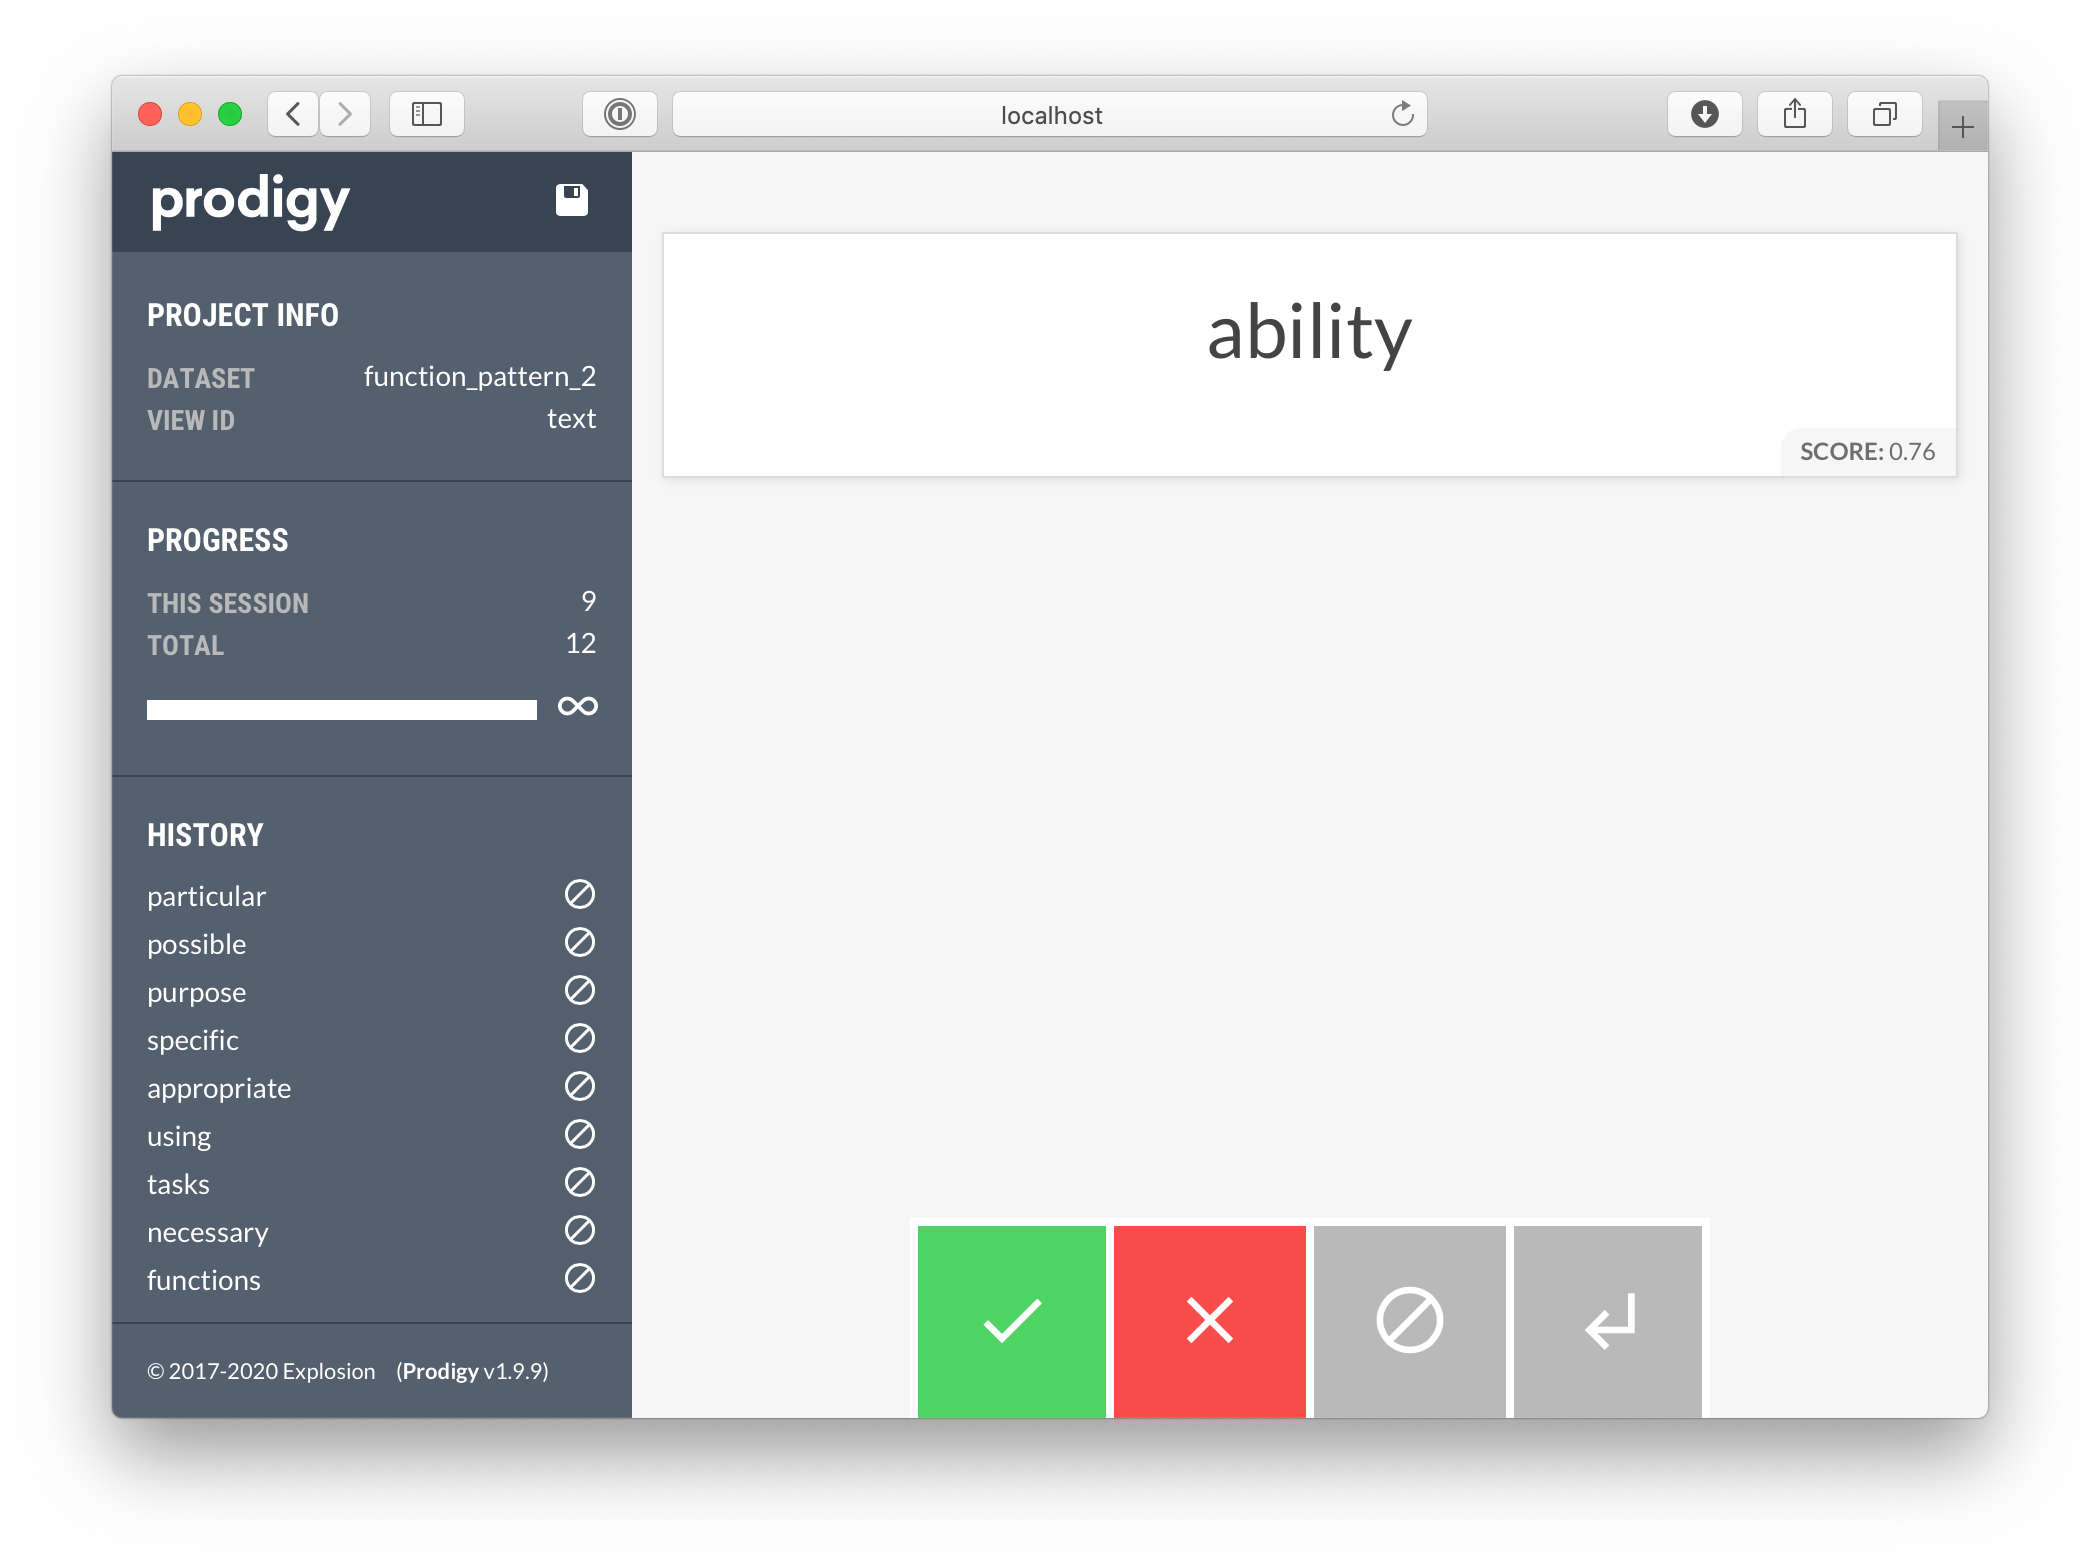
\includegraphics[width=1.19\linewidth]{fig11.png}
  \caption{Prodigy training tool installed in a local developer environment}
  \label{fig:figure11}
\end{figure}
\vspace*{1.2em}

The terms.teach recipe uses word2vec and delivered promising results.
We expected to get better results using sense2vec through the textcat.teach recipe and a new format for seed terms using JSON (a file format for human-readable data objects) instead of plain text.
Seed terms in sense2vec can be initialised using their parts-of-speech, so we can compare results using our focus words as nouns instead other parts that the algorithm identifies in our corpus.
However, we did not get this to work as there are more files required for sense2vec to function.
Simply loading the new seeds as JSON produced errors and loading the seeds from the plain text file assigned verb as a POS for use.
Furthermore, the only corpus that worked out-of-the box with the sense2vec model was Reddit.
Reddit includes the required vectors that are either missing or in a wrong format using en\_core\_web\_lg, making a straight comparison with the word2vec model difficult.

%===================================

\section{Comparison of results}

We compiled results from all above tools into a table (Table \ref{fig:table5}).
From this comparison we can identify certain patterns regarding the context of the words and to an extent understand the effect of a corpus or algorithm on the results.

It can be seen that some words are found in almost every tool while others are unique to a single one.
There are also many repetitions of word stems and lemmas which speaks for poor data preprocessing.

\vspace*{1.2em}
\begin{figure}[!htbp]
  \hspace*{-3.666em}
  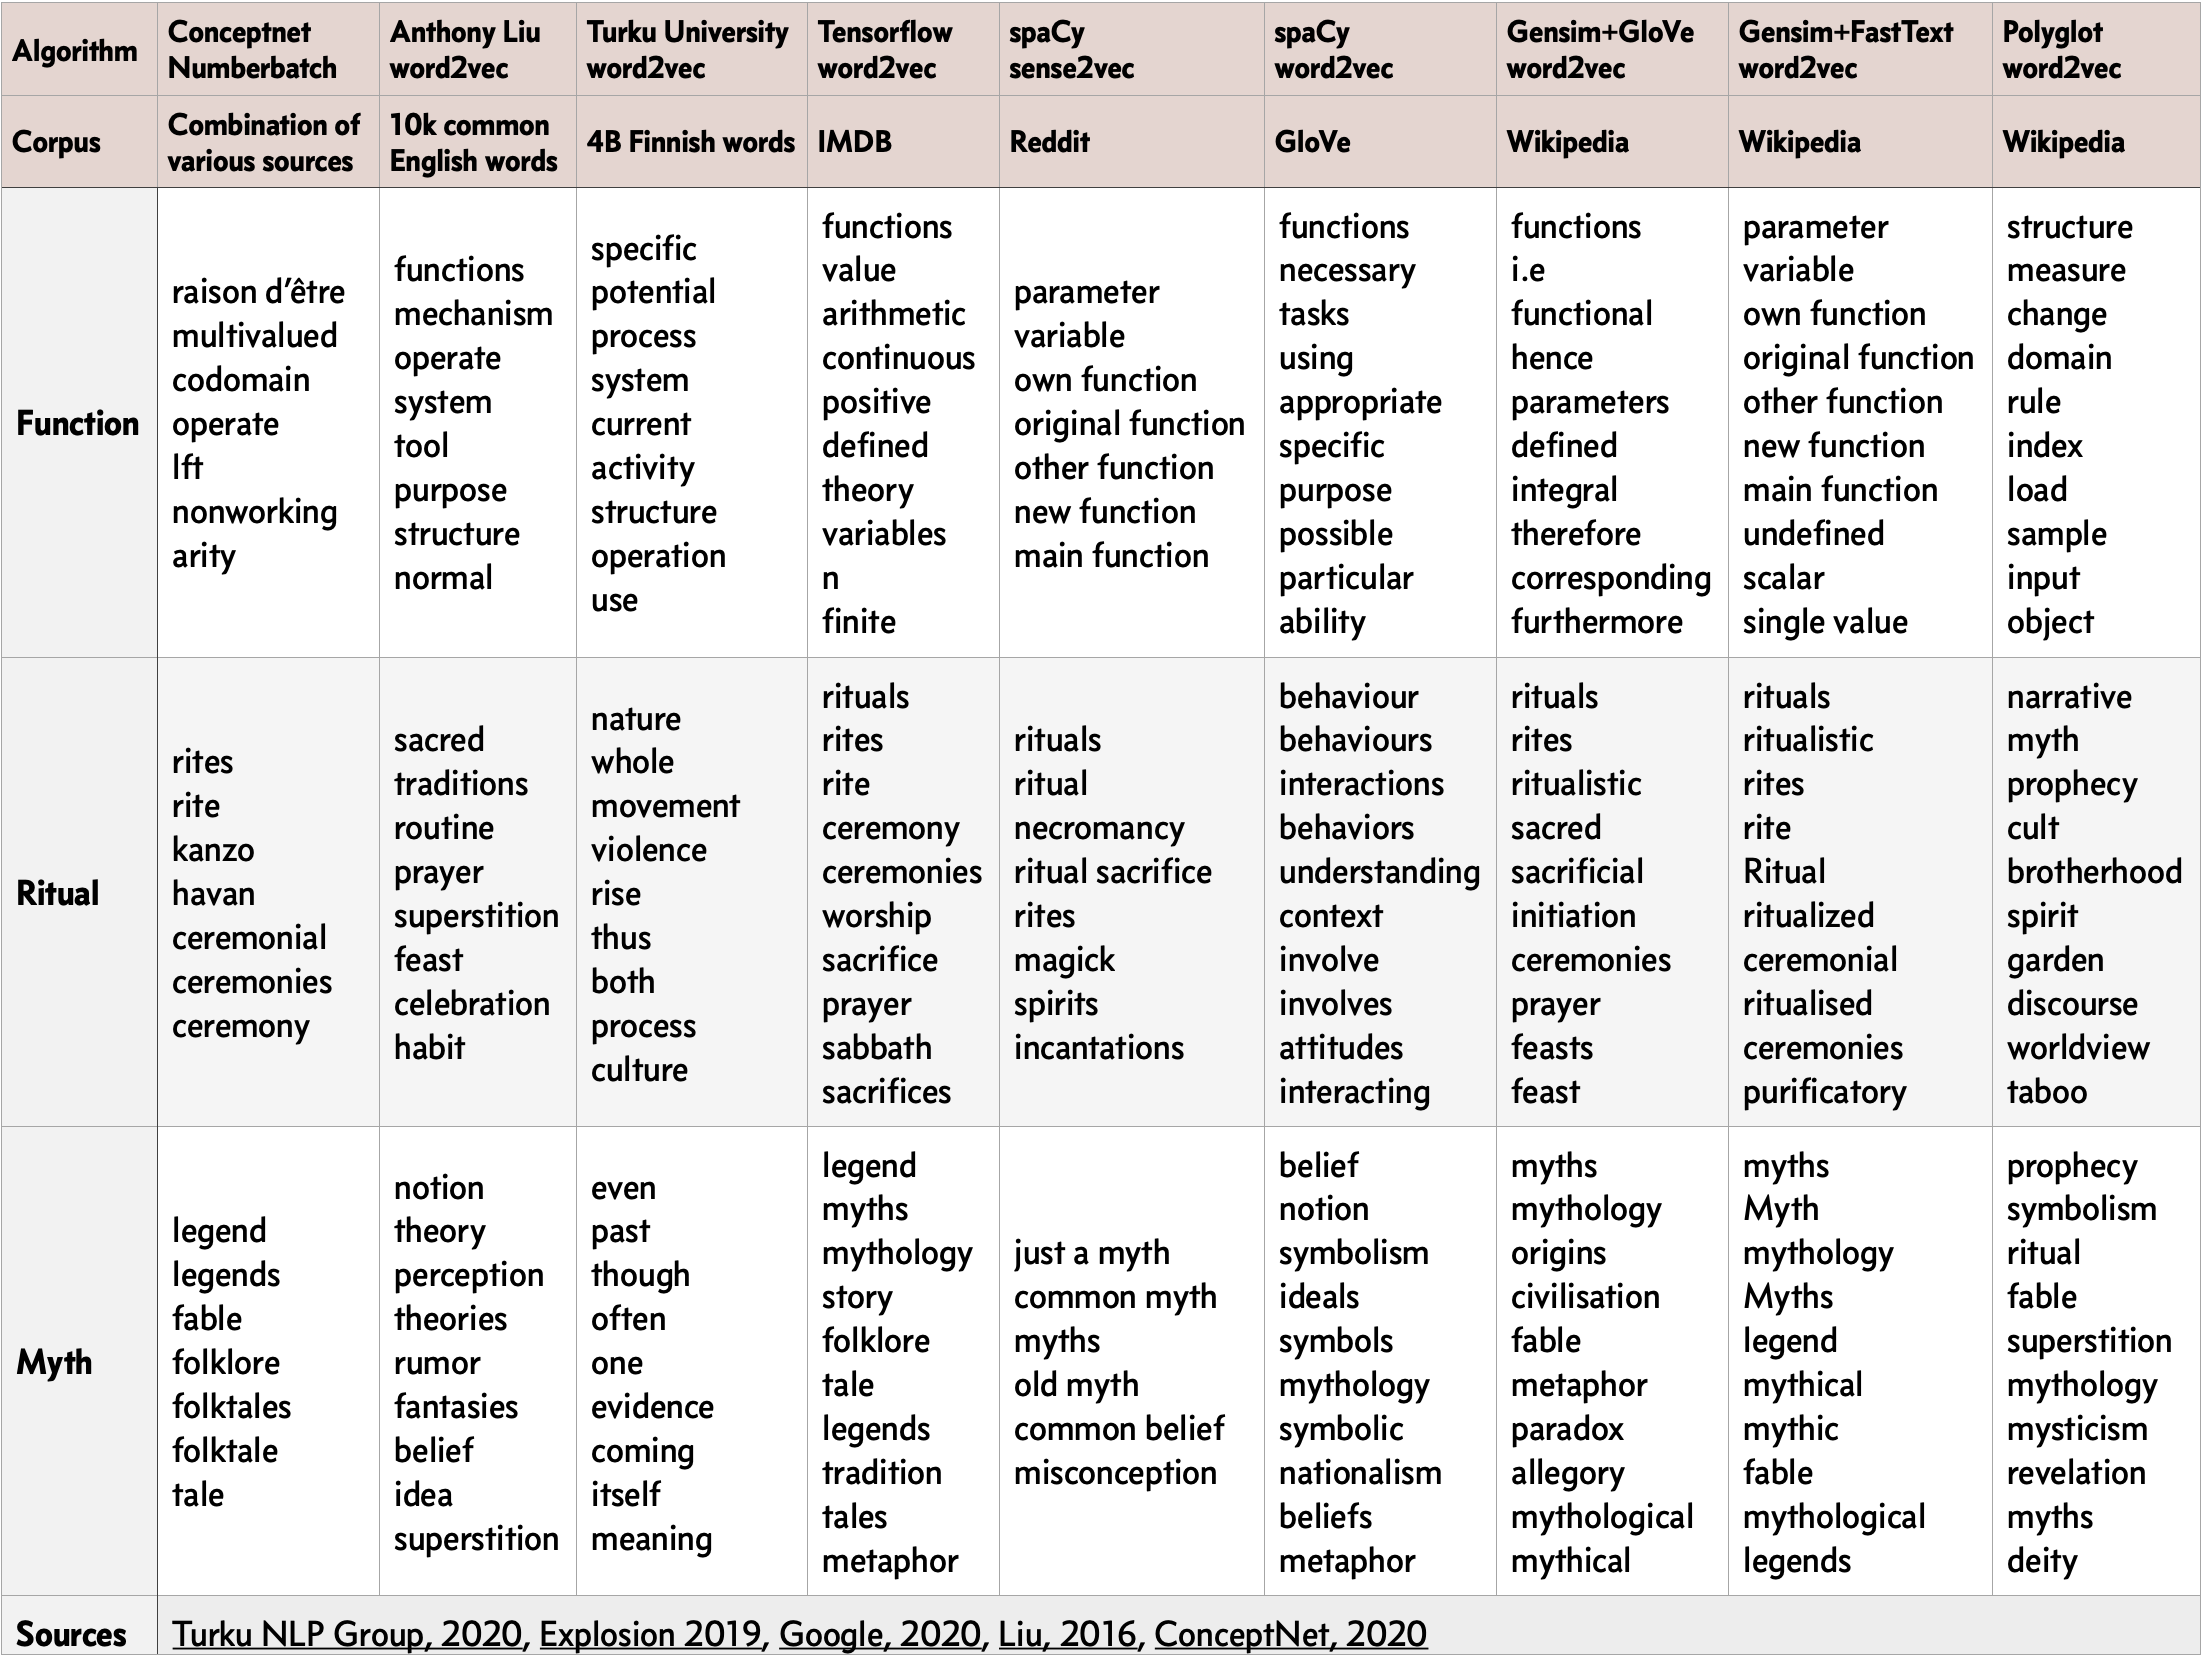
\includegraphics[width=1.19\linewidth]{table5.png}
  \caption{Results from online demos and local scripts using different algorithms and corpora}
  \label{fig:table5}
\end{figure}
\vspace*{1.2em}

Function often exists in the context of computer science, which is not surprising given the field of NLP is one of artificial intelligence, machine learning, data analysis, and formulas.
Parts of computer programs are called functions, and as such we can expect many derivations of the term either as part of a program or just function as the name for a function.
In ConceptNet we can find the word used in the acronym LFT (liver function test) from the field of medicine and arity which comes from mathematics.
It is curious that the IMDB corpus also outputs technical uses of function such as variables or n, which presumably stands for number.
While we do not have exact criteria to rank these results, the output from Polyglot has the most range and fewest repetition of computer science terms.

Ritual was often associated with ceremonial topics and religion.
While there is a certain celebration in the ritualisation of using an object, religion is not the context we intended to evoke.
Tradition, routine and habit found in Anthony Liu’s demo using common English words are more in line with the aspect of social interaction identified by Giacomin (2017) \cite{giacomin2017}.
It can also be observed that spellings of British English and American English are interpreted uniquely, which is in line with the function of word2vec where each morphological structure of a word is assigned their own vector.
We did not sanitise the table by removing these duplicates since they were not identified as such by the machine even though to us they clearly are.
Myth is associated with fairytales, fables, folklore, made-up fantasies and misconception.
Two instances of symbolism can be found in SpaCy with GloVe and Polyglot with Wikipedia.
This finding was interesting as it closes the loop of this document by returning to Susan Fournier’s \ref{fig:function-symbolic} axis of mapping object meanings from functional to symbolic.

%===================================

\section{Current Conclusions}

Regarding our selection of SpaCy paired with Prodigy as the focus, it cannot be ruled out that this combination is still the “winner”, but it is clear that we made mistakes in the application of the tools.
In contrast, the results from the Polyglot demo are the most promising in Table \ref{fig:table5}. 
We have breadth of context without repetitions and are rediscovering symbolism as a potential alternative to myth, which is negatively loaded.

When we used Prodigy with one one seed term (function), the results we saw were exactly the same as those using Gensim+FastText using GloVe.
Both libraries share GloVe and word2vec. Similarity can be expected, a mirror image was surprising.
The results found in Table \ref{fig:table5} are using three seed words.
We also tried 15 seed terms and these were our results: other functions, main function, method, other function, specific function, multiple functions, constraint, certain function.
It is unclear what conclusions we can draw from this.

While there is good documentation available for NLP tools, the field itself is still foreign to us and we have only scratched the surface in understanding the different concepts and are unfamiliar with Python programming.
We focused on Prodigy because it offers text classification and training in a graphical user interface, and put the online demos aside since they are not trained on our context.
In hindsight we should have spent more time looking at the existing demos because we did not achieve the desired training and corpus-comparison using Prodigy.

%===================================

\section{Next Steps}

The combination of Prodigy and SpaCy was interesting to us for one more reason: the trained model can be imported into Tensorflow and visualised in its 3D vector-space.
We did not get to that stage and wish to do this at a later point.
To produce results for the import, we want to revisit ou training and have another the vector files to see if all features (lemmatisation, stemming, polysemy, etc.) are enabled, and to control POS for seed terms.
We also want to try another corpus for training and see if the model finds more diverse and less repetitive results.

The output from Table \ref{fig:table5} will have to be evaluated by non-experts and compared to the dictionary results.

In the next document, we will need to get back to the bigger picture of defining Design for Meaning.
In this publication we focused on NLP and assumed some prior knowledge of the works by Csikszentmihalyi and Rochberg-Halton (1981), or more recently by Crilly, Maier, and Clarkson (2008), Diller, Shedroff and Rhea (2008) or Gobé (2009).

The plan for the next phase of this project is as follows:

\begin{enumerate}
	\item Compare and contrast Table 5 with Table 1 and potentially compile a comprehensive merged version
	\item Build a survey of words to send out to testers and evaluate which words resonate most with people. Get input from people on words that they think are missing from the table.
	\item While waiting on results from the survey, we can have another look at NLP
	\item Re-evaluate the word associations
	\item Build a new survey where we have people classify familiar products into the three categories of meaning, using our new word list.
	\item Evaluate and identify potential patterns
\end{enumerate}

%===================================

\chapter{Contextualisation}

\section*{Introduction}

We pick up where we left off. Compare to the plan made in June. We researched on context (Automotive Cars), made two surveys.

todo
\begin{itemize}
	\item add references for websites to bibliography
	\item justify AV context
	\item design final test
	\item words, enhanced with images
	\item examples of function, ritual and myth in vehicles (giacomin)
\end{itemize}

%===================================

\section{Context: Automotive Vehicles}

%===================================

\section{Survey 1: Word Meaning}

%===================================

\section{Survey 2: Image Association}

%===================================

\section{Survey Results}

%===================================

\section{Identifying Patterns}

%===================================
%===================================

\bibliography{d4mbib}
\bibliographystyle{ieeetr}

\end{flushleft}
\end{document}
